%% LyX 2.1.4 created this file.  For more info, see http://www.lyx.org/.
%% Do not edit unless you really know what you are doing.
\documentclass[a4paper,ngerman,naustrian,DIV=12,BCOR=1cm]{scrbook}
\usepackage[T1]{fontenc}
\usepackage[utf8]{inputenc}
\usepackage{fancyhdr}
\pagestyle{fancy}
\setcounter{secnumdepth}{3}
\usepackage{babel}
\usepackage{textcomp}
\usepackage{url}
\usepackage{makeidx}
\makeindex
\usepackage{graphicx}
\PassOptionsToPackage{normalem}{ulem}
\usepackage{ulem}
\usepackage[unicode=true,
 bookmarks=true,bookmarksnumbered=false,bookmarksopen=false,
 breaklinks=true,pdfborder={0 0 0},backref=false,colorlinks=false]
 {hyperref}
\hypersetup{pdftitle={Hovering Steward},
 pdfauthor={Christina Bornberg, Katharina Joksch, Markus Kaiser, Alexander Punz, Lucas Ullrich},
 pdfsubject={Diplomarbeit},
 pdfkeywords={project,hexacopter,multicopter,drone,hovering,steward,autonomous,flying,blog,HTL,rennweg,event,cupcakes,restaurant,vienna,austria,technology,research}}

\makeatletter

%%%%%%%%%%%%%%%%%%%%%%%%%%%%%% LyX specific LaTeX commands.
\pdfpageheight\paperheight
\pdfpagewidth\paperwidth

%% Because html converters don't know tabularnewline
\providecommand{\tabularnewline}{\\}

%%%%%%%%%%%%%%%%%%%%%%%%%%%%%% Textclass specific LaTeX commands.
\newcommand{\strong}[1]{\textbf{#1}}
\newcommand{\code}[1]{\texttt{#1}}

%%%%%%%%%%%%%%%%%%%%%%%%%%%%%% User specified LaTeX commands.
%%%%%%%%%%%%
% Latex-Vorspann
\usepackage{lastpage}
\usepackage{listings}
\usepackage{blindtext}

%% geht nicht mit jeder Latex Variante, gibt aber ein schöneres Layout
\usepackage{microtype} 

%% Aufzählungen nicht so weit einrücken
\usepackage{enumitem}
%\setitemize{leftmargin=*} 

%\usepackage{caladea}
%\usepackage[T1]{fontenc}
\usepackage{lmodern}

\usepackage{xspace}

%% für pandoc
%% maximale Breite der Bilder
\usepackage{graphicx}
\setkeys{Gin}{width=0.90\linewidth,keepaspectratio}
\providecommand{\tightlist}{%
\setlength{\itemsep}{0pt}\setlength{\parskip}{0pt}}

%%für Bilder nebeneinander
\usepackage{subfigure}

%um Schusterjungen und Hurenkinder vermeiden zu können
\usepackage{needspace}

%Farbpaket
\usepackage{xcolor}

\usepackage{float}

\usepackage{setspace}
\spacing{1.3}

\makeatother

\usepackage{listings}
\addto\captionsnaustrian{\renewcommand{\lstlistingname}{\inputencoding{latin9}Listing}}
\addto\captionsngerman{\renewcommand{\lstlistingname}{\inputencoding{latin9}Listing}}
\renewcommand{\lstlistingname}{\inputencoding{latin9}Listing}

\begin{document}
%%%%%%
% Weitere Einstellungen siehe Latex-Vorspann

\sloppy % weniger Meldungen

\voffset5mm % etwas nach unten%%%%%%%%%%%%%%%%%%%%%%%%%%%%%%%%%%%%%%%%%%%%%%%%%%%%%%%%%%%%%%%%%%%%%%%%%%%%%%%%%%
% falls man die erste Zeile der Absätze nicht einrücken will
% dann sollte man aber etwas mehr Abstand zwischen den Absätzen erlauben
% Alternative \usepackage{parskip}
%%\setlength{\parindent}{0pt}
%%\setlength{\parskip}{1.5ex plus0.5ex minus0.5ex}
% Auch Fußnoten bündig ausrichten
\deffootnote[]{1em}{1em}{\textsuperscript{\thefootnotemark\ }}
% Listen etwas wenige einrücken, erfordert enumitem
\setitemize{leftmargin=*}

%%%%%%%%%%%%%%%%%%%%%%%%%%%%%%%%%%%%%%%%%%%%%%%%%%%%%%%%%%%%%%%%%%%%%%%%%%%%%%%%%%
%  Kopf und Fußzeilen -- links und rechts verschieden 
\newcommand{\kopfseitenummer}{{\bfseries \thepage}}
\newcommand{\kopfkapl}{{\bfseries\leftmark}}
\newcommand{\kopfkapr}{{\bfseries\rightmark}}
\newcommand{\kopfbild}{
\includegraphics[width=25mm]{HTL3RLogoRGB}}
\newcommand{\kopfHTL}{Höhere Technische Bundeslehranstalt Wien 3, \\Rennweg 	Abteilung für Informationstechnologie}
\renewcommand{\chaptermark}[1]%
  {\thispagestyle{fancy}\markboth{\thechapter.\ #1}{}}%\thispagestyle{fancy}

%\lhead[\fancyplain{\kopfbild}{\kopfbild}]% li aussen
%      {\fancyplain{\kopfHTL}{\kopfHTL}}% re innen
%\rhead[\kopfHTL]% li innen
%      {\kopfbild}% re aussen

%% mit kapitelautor kann man den Autor festlegen oder auf leer setzen - steht dann in der Fußzeile.
\newcommand{\kapitelautor}{}

%%%
% Alternative: am Rand (Marginale)
%\setlength{\marginparsep}{-5mm}
%\mbox{}\marginpar{\raggedleft\hspace{0pt}Autor: Hans Huber}

%% kopf links: [linke] und {rechte} Seite
\lhead[\kopfbild]{\kopfkapl}
\rhead[\kopfkapr]{\kopfbild}
\chead{}

\lfoot[\kopfseitenummer]{\kapitelautor}
\cfoot[]{}
\rfoot[\kapitelautor]{\kopfseitenummer}
\renewcommand{\footrulewidth}{0.2pt}
\renewcommand{\headrulewidth}{0.2pt}

%%
% einfaches "siehe ..." - das Ziel muss man markieren
\newcommand{\kap}[1]{Kapitel~\ref{#1}, Seite~\pageref{#1}}
\newcommand{\siehe}[1]{siehe \kap{#1}}

%% http://ieg.ifs.tuwien.ac.at/~aigner/download/tuwien.sty
%Div. Abkürzungen (in Anlehnung an Jochen Köpper, jkthesis):
%\RequirePackage{xspace}
\newcommand{\bzw}{bzw.\@\xspace}
\newcommand{\bzgl}{bzgl.\@\xspace}
\newcommand{\ca}{ca.\@\xspace}
\newcommand{\dah}{d.\thinspace{}h.\@\xspace}
\newcommand{\Dah}{D.\thinspace{}h.\@\xspace}
\newcommand{\ds}{d.\thinspace{}s.\@\xspace}
\newcommand{\evtl}{evtl.\@\xspace}
\newcommand{\ua}{u.\thinspace{}a.\@\xspace}
\newcommand{\Ua}{U.\thinspace{}a.\@\xspace}
\newcommand{\usw}{usw.\@\xspace}
\newcommand{\va}{v.\thinspace{}a.\@\xspace}
\newcommand{\vgl}{vgl.\@\xspace}
\newcommand{\zB}{z.\thinspace{}B.\@\xspace}
\newcommand{\ZB}{Zum Beispiel\xspace} 

%%%%%Anfang Titelseite
\pagenumbering{roman}
\title{Diplomarbeit}
\begin{titlepage}
\begin{minipage}[b]{1\columnwidth}
\parbox[b]{50mm}{
\includegraphics[width=45mm]{HTL3RLogoRGB}}
\hfill
\parbox[b]{130mm}{\footnotesize \textsc{Höhere Technische Bundeslehranstalt} Wien 3, Rennweg\\
IT \& Mechatronik\\
\\
HTL Rennweg :: Rennweg 89b\\
A-1030 Wien :: Tel +43 1 24215-10 :: Fax DW 18
}\\
\mbox{}
\end{minipage}

\vspace{1cm}


\begin{center}
\textbf{\LARGE{}Diplomarbeit}{\large{}}\\
{\large{}\vspace{15mm}
 }\textbf{\large{}}\\
\textbf{\large{}Hovering Steward}\\
 \vspace{15mm}
 ausgeführt an der\\
 Höheren Abteilung für Informationstechnologie/Ausbildungsschwerpunkt\\
 der Höheren Technischen Lehranstalt Wien 3 Rennweg\\
 \vspace{1cm}
 im Schuljahr 2015/2016\\
 \vspace{1cm}
 durch\\
 \vspace{0.5cm}
\textbf{\large{}Christina Bornberg}\\
\textbf{\large{}Katharina Joksch}\\
\textbf{\large{}Markus Kaiser}\\
\textbf{\large{}Alexander Punz}\\
\textbf{\large{}Lucas Ullrich}\\

\par\end{center}{\large \par}

\begin{center}
\vspace{20mm}
\normalsize unter der Anleitung von\\
\vspace{0.5cm}
Mag. Andreas Fink\\
DI Herbert Fleck
\par\end{center}

\begin{center}
\vspace{5mm}
Wien, \today 
\par\end{center}

\end{titlepage}%%%%%%%%%%%%%%%%%%%%% Ende Titelseite %%%%%%%%%%%%%%%%%%%%%

\renewcommand*{\chapterpagestyle}{fancy}

%%%%%Programmlisting%%%%%%%%
% das braucht man nur einmal
\lstset{basicstyle = \ttfamily\footnotesize,
	keywordstyle = \color{blue},
	stringstyle = \color{cyan},
	commentstyle = \color{lightgray},
	numbers = left,
	numberstyle = \tiny,
	stepnumber = 2, 
	numbersep = 5pt, 
	showspaces = false, 
	frame = single,
	escapechar = $
}
%lstset{language=...} vor jedem Listing

%hier geht es los mit dem Text - auf einer rechten Seite
\pagenumbering{arabic}
\pagestyle{fancy}
\thispagestyle{fancy} 

%\renewcommand{\kapitelautor}{Autor: VN NN} immer im Unterdokument

\thispagestyle{fancy}

% !TEX root = diplomarbeit.tex
\chapter{Einleitung}
\renewcommand{\kapitelautor}{Autor: Markus Kaiser}

%%%%%%%%%%%%%%%%%%%%%%%%%%%%%%%%%%%%%%%%%%%%%%%%%%%%%%%%%%%%%%%%%%%%%%%%%%%%%%%
\section{Projektidee}
Die Idee des Projektes, ist die Entwicklung einer Konzeptstudie eines innovativen Logistiksystems, das sich durch die Verwendung eines Multicopters auszeichnet.
Für den Entwicklungsprozess im Zuge der Diplomarbeit wurde die Gastronomie als Einsatzbereich gewählt. Diese Wahl ermöglich zum einen
ein konkreteres Fomulieren der Ziele und zum anderen eine einheitliche Vision innerhalb des Teams.

Der innovative Aspekt des Projekts wird insofern abgedeckt, dass die Entwicklung des Systems so durchgeführt wird,
dass es auch in anderwärtigen Bereichen der Logistik, wie beispielsweise der Lagerverwaltung eingesetzt werden kann.

Das System setzt sich aus den folgenden drei Komponenten zusammen:

\begin{itemize}
  \item Multicopter
  \item Firmware
  \item Digitale Speisekarte
\end{itemize}

\begin{figure}[H]
  \begin{centering}
  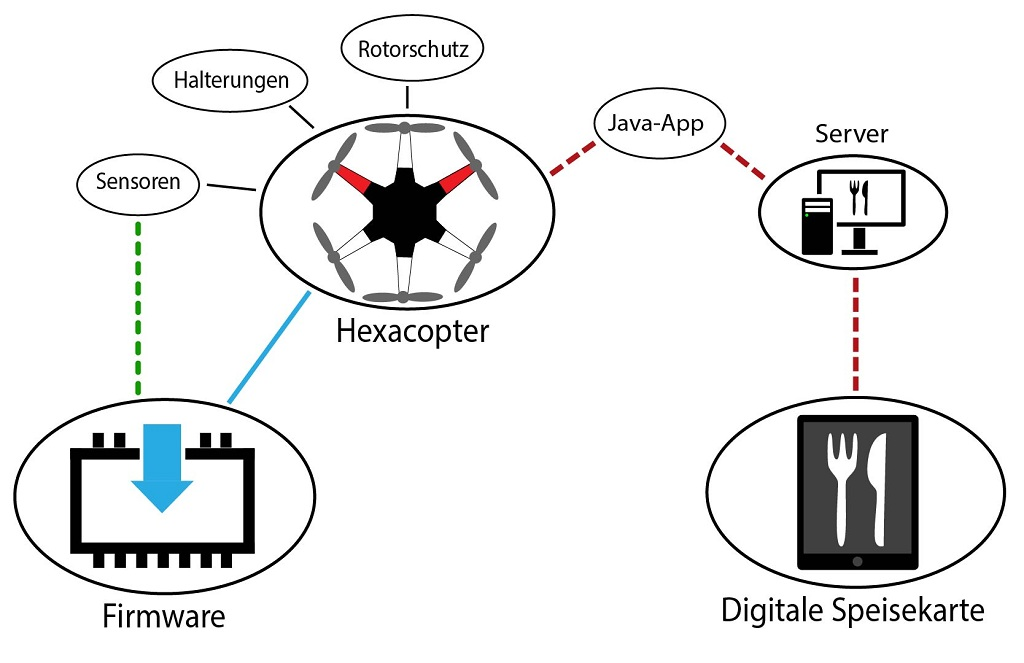
\includegraphics[width = 0.9\textwidth]{Bilder/systemblockbild.jpg}
  \par\end{centering}
  \caption{Systemblockbild}
  \label{Systemblockbild}
\end{figure}

Der Multicopter ist die zentrale Komponente des Projekts. Er ist für den selbstständigen Transport von Objekten zuständig,
und muss somit flugfähig, und im Stande sein Unfälle zu verhindern. Sensoren, die mittels eigens angefertigter Halterungen
am Multicopter befestigt sind, kommunizieren mit der Firmware.

Die Firmware regelt alle logischen Prozesse des Systems. Sowohl die Steuerung des Multicopters, als auch der
Austausch von Daten fällt unter diese Kategorie. Befehle erhält sie unter anderem von der Speisekarte, mit der sie über
einen Server, beziehungsweise einer weiteren Anwendung kommuniziert.

Die digitale Speisekarte ist indirekt die externe Steuereinheit des Multicopters, und zugleich die Komponente,
die das System für den Einsatz in der Gastronomie auszeichnet. Sie automatisiert Vorgänge eines gastronomischen
Betriebs und wandelt Nutzereingaben in Befehle für den Muticopter um.

%%%%%%%%%%%%%%%%%%%%%%%%%%%%%%%%%%%%%%%%%%%%%%%%%%%%%%%%%%%%%%%%%%%%%%%%%%%%%%%
\section{Ausgangssituation}
  In den folgenden Absätzen wird beschrieben, wie die Idee von Hovering Steward, dem autonom fliegenden Kellner
  entstanden ist, und womit sich die ersten Recherchen zu Begin des Projektes beschäftigt, beziehungsweise
  welche Ergebnisse diese hervorgebracht haben.

  \subsection{Ideenfindung}
  Ihren Anfang fand die Idee im Projektmanagement Unterricht. Klasseninterne Teams mussten ein fiktives Projekt erfinden, um auf Basis dieses
  Projektmanagementpläne zu erstellen. Es entstand "Fluorescent Bakery", eine Bäckerei, die fluoreszierende Cupcakes verkauft.
  Der technische Teil ergab sich später, bei dem Gedanken diese Idee für die Diplomarbeit weiterzuverwenden. Der Ansatz hierfür war,
  einen nicht menschlichen Kellner zu erschaffen, der selbstprogrammiert, die Aufgaben einer Bedienung in einem Restaurant übernimmt.
  So entstand "Hovering Steward - der autonom fliegende Kellner", ein dreidimensionales "Tracking-System", welches eine Drohne in einem Raum die Aufgaben eines Kellners durchführen lässt.
  Das Projekt erhielt später noch eine weitere Komponente, nämlich eine digitale Speisekarte, um das automatische System zu erweitern.

  \subsection{Stand der Technik}
  \subsection*{Themenrestaurants}

  \begin{itemize}
    \item \textbf{Disaster Café}

    Das Themenrestaurant {Disaster Café\cite{disastercafe}} in Spanien bietet Gästen die Erfahrung, ihr Essen bei einem Erdbeben
    der Stärke 7.8 zu sich zu nehmen.

    \item \textbf{Das stille Örtchen - Modern Toilet}

    Eingerichtet wie eine Toilette, können Gäste des {Modern Toilet\cite{moderntoilet}} in Japan ihre Speisen in einem gewohnten Umfeld genießen.

    \item \textbf{Affen-Kellner}

    {Eine kleine Taverne in Japan\cite{affenkellner}} besitzt zwei kleine Affen, die Tätigkeiten wie das Servieren von Getränken oder Handtüchern
    für den Inhaber übernehmen. Sie verstehen sogar, welche Getränke ein Gast bestellt.

    \item \textbf{The Royal Dragon}

    Neben Rollschuh fahrenden Kellnern verfügt das weltweit größte {Restaurant für Meeresfrüchte\cite{royaldragon}} eine
    Art Seilbahn, mit der ein Kellner "fliegend" das Essen serviert.

    \item \textbf{Dinner in the Sky}

    Bei {Dinner in the Sky\cite{dinnerinthesky}} werden die Gäste samt Tisch und kleiner Küche von einem Kran 50 Meter
    in die Luft gezogen, wo dann gespeist wird.

    \item \textbf{Dinner in the Dark}

    In diesem {Themenrestaurant\cite{dinnerinthedark}} verbringen die Gäste ihren Aufenthalt im Dunkeln. Einzig und allein die
    Kellner können mittels Nachtsichtbrille etwas sehen.

  \end{itemize}

  \subsection*{Multicopter in der Gastronomie}
  \begin{itemize}
      \item \textbf{Infinium-Serve}

      Das Unternehmen {Infinium-Robotics\cite{infiniumserve}} hat ein System entwickelt, welches Gästen eines Restaurants
      das Essen mittels Hexacopter serviert.

      \item \textbf{iTray}

      {iTray\cite{itray}}, ein Projekt aus London, nutzt kleine Drohnen um Sushi an die Tische der Gäste zu bringen.
      Die Drohnen werden über ein Remote-Wi-Fi-System gesteuert.

  \end{itemize}

  \subsection*{Multicopter Projekte}
  \begin{itemize}
      \item \textbf{ETH Flying Machine Arena}

      Die {"Flying Machine Arena"\cite{eth}} ist ein portables System, welches einen virtuellen Raum mit den Maßen 10x10x10 Meter aufbaut, in welchem
      Objekte mit hoher Präzision erkannt und verfolgt werden können. Das System ist für Experimente mit autonom fliegenden Hexacoptern
      gedacht, die sich in diesem virtuellen Raum über drahtlose Kommunikation orientieren können.

      \item \textbf{Lily}

      {Lily\cite{lily}} ist eine selbstständig fliegende Drohne mit eingebauter Kamera. Ihr Zweck ist, dass sie den Benutzer auf seinem Weg verfolgt.
      Sie wird dafür einfach in die Luft geworfen, worauf sie sich stabilisiert. Danach folgt sie dem Benutzer in einem festgelegten Abstand, solange dieser ein, für Lily
      vorgesehenes Armband trägt und filmt mit einer HD Kamera alles mit.

      \item \textbf{DHL Paketcopter}

      Der {DHL Paketcopter\cite{dhl}} ist ein Innovationsprojekt der DHL, bei dem ein Paket per Drohne zugestellt wird. Die Drohne ist in der Lage große Strecken zu fliegen,
      und somit auch zu schwer erreichbaren Orten zu gelangen, wenn Menschen dazu keine Möglichkeit mehr haben. Auf der Insel Juist wird sie beispielsweise als
      Medikamentenversorger verwendet, da am Wochenende keine Lieferungen per Schiff auf die Insel zugestellt werden.

      \item \textbf{Ambulance Drone}

      Die {Ambulance Drohne\cite{ambulancedrone}} ist ein Projekt, welches auf der TU Delft entwickelt wird. Das Besondere an dieser Drohne ist, dass sie einen eingebauten Defibrillator hat, welcher
      sich per Fernverbindung von einem Rettungshelfer bedienen lässt, obwohl dieser nicht anwesend ist. Die Ambulance Drohne fliegt mit einer Höchstgeschwindigkeit von bis zu
      100 Stundenkilometer und kann somit, in einem Notfall, schnell die Unfallstelle erreichen.

      \item \textbf{Gimball}

      {Gimball\cite{gimball}} ist der weltweit erste fliegende Roboter, der immun gegen Kollistionen ist. Seine Konstruktion besteht aus einem kugelförmigen Gerüst, in dem die Drohne
      aufgehängt ist, und sich anhand von Gelenken trotzdem frei darin bewegen kann. Die Kugel fängt Stöße ab, wodurch die Drohne ungehindert an schwer erreichbare
      Orte gelangt.

  \end{itemize}

%%%%%%%%%%%%%%%%%%%%%%%%%%%%%%%%%%%%%%%%%%%%%%%%%%%%%%%%%%%%%%%%%%%%%%%%%%%%%%%
\section{Team und Aufgabenverteilung}
  \subsection*{Markus Kaiser}
  \textbf{Projektleitung und Marketing}

  Markus Kaiser leitete das Team Hovering Steward und war somit für das Projektmanagement und
  die organisatorischen Aspekte verantwortlich. Neben dieser Hauptrolle zählte außerdem das Marketing
  zu seinen Aufgabenbereichen, was speziell die Entwicklung des Blogs anbelangte. Durch seine Kenntnisse
  in der Webentwicklung stellte er mit dem Blog eine wichtige Schnittstelle zur Außenwelt her.

  \subsection*{Lucas Ullrich}
  \textbf{Sensorik \& Firmware}

  Lucas Ullrich war neben seiner Position als Projektleiter Stellvertreter für die Sensorik an unserer Drohne und
  für die Programmierung der Firmware zuständig. Er unterstützte unseren Projektleiter bei terminlichen Angelegenheiten
  und konnte durch seine Kenntnisse mit der Programmiersprache C eine solide Basis für die Firmware des Microcontrollers schaffen.
  Außerdem entwarf er die Schaltpläne, und erstellte somit ein Konzept für die Sensorik.

  \subsection*{Christina Bornberg}
  \textbf{Firmware}

  Christina Bornberg fungierte als Firmware Entwicklerin des Teams. Durch ihre Interesse an der Programmierung von Drohnen
  und bereits gesammelten Erfahrung mit der Programmierung von C konnte sie gemeinsam mit Lucas Ullrich die erarbeiteten Konzepte hinter
  dem automatisierten Flug der Drohne in Code realisieren.

  \subsection*{Katharina Joksch}
  \textbf{Webentwicklung}

  Der Aufgabenbereich von Katharina Joksch war die Webentwicklung, genauer gesagt die Programmierung der digitalen Speisekarte.
  Neben der Planung der Datenbank und der sinnvollen Verwendung hilfreicher Frameworks entwickelte sie außerdem eine Java Applikation,
  die die Kommunikation zwischen der digitalen Speisekarte und der Drohne regelte.

  \subsection*{Alexander Punz}
  \textbf{Hardware \& Mechanik}

  Alexander Punz war sowohl für die Hardware, als auch für die Mechanik verantwortlich. Seine Aufgaben waren sowohl die Konzeption
  und Produktion des Rotorschutzes, der einen sicheren Flug der Drohne ermöglichte, als auch die Herstellung diverser Halterungen,
  die für Sensorik, Transport und Flugtests verausgesetzt waren.

%%%%%%%%%%%%%%%%%%%%%%%%%%%%%%%%%%%%%%%%%%%%%%%%%%%%%%%%%%%%%%%%%%%%%%%%%%%%%%%
\section{Betreuer}
  \subsection*{Mag. Andreas Fink}
  Mag. Andreas Fink stand dem Projektteam als Hauptbetreuer der Abteilung für Informationstechnologie zur Seite.
  Seine objektive Sichtweise auf das Projekt, hat dem Team sehr geholfen den Fokus auf die Ziele zu legen und
  das Projekt in die Richtung zu entwickeln.
  Zusätzlich dazu betreute er individuell Markus Kaiser bei den Aspekten Projektleitung und Marketing.

  \subsection*{DI Herbert Fleck}
  DI Herbert Fleck war Hauptbetreuer der Mechatronik Abteilung unseres Teams. Er koordinierte den Prozess der Diplomarbeit
  gemeinsam mit Mag. Andreas Fink. Das Team schätzte außerdem sehr das konstruktive Feedback bei Präsentationen.
  Er betreute nebenbei Lucas Ullrich mit Fachwissen aus dem Bereich der Elektronik.

  \subsection*{DI August Hörandl}
  DI August Hörandl fungierte als Individualbetreuer von Christina Bornberg. Duch seine Fähigkeiten und
  Erfahungen als Programmierer sowohl mit der Sprache C, als auch Java war das Entwickeln der Firmware,
  aber auch der Java-Applikation für die WLAN-Kommunikation wesentlich einfacher. Außerdem war
  DI August Hörandl unser Ansprechpartner wenn es Unklarheiten bei \LaTeX gab.

  \subsection*{MMag. Florian Weiss}
  MMag. Florian Weiss betreute Katharina Joksch bei der Entwicklung der digitalen Speisekarte. Sein umfangreiches
  Know-How im Bereich der Webentwicklung, dem Umgang mit diversen Frameworks und Bibliotheken half Katharina
  dabei ein Grundgerüst für die Entwicklung aufzubauen.

  \subsection*{DI Franz Temper}
  DI Franz Temper unterstützte Alexander Punz bei der Entwicklung der Konstruktionen. Durch Fachwissen mit
  der Software Creo und Unterstützung bei 3D-Druck war es möglich, dass Alexander alle seiner Ziele erfolgreich
  umsetzen konnte.

%%%%%%%%%%%%%%%%%%%%%%%%%%%%%%%%%%%%%%%%%%%%%%%%%%%%%%%%%%%%%%%%%%%%%%%%%%%%%%%
\section{Partner / Sponsoren}

\subsection*{GRZ IT Center GmbH}
{GRZ IT Center\cite{grz}} ist eines der größten Rechenzentren österreichs. Mit dem Fokus auf Bankenservicierung arbeitet das Unternehmen
mit Partnern wie Raiffeisen zusammen. Auf eine Anfrage für ein Sponsoring der Diplomarbeit erhielten wir die überaschende
Antwort, dass GRZ das Projekt sehr interessant findet, und uns aus diesen Gründen als Hauptsponsor, mit einem beträchtlichen Betrag
unterstützen würde.
Es wurde ein Sponsoringvertrag, auf Basis einer Mustervorlage aufgesetzt, in welchen beidseitig Konditionen für die Partnerschaft
verfasst wurden, und von beiden Parteien unterzeichnet.

\subsection*{OFI}
{Das Österreichische Forschungsinstitut\cite{ofi}} ist Experte die Prüfung für Werkstoffanwerundung
und Bauwerkserneuerungen. Neben finanzieller Unterstützung erhielt das Projektteam
ein professionelles, projektbegleitendes Team-Coaching, inklusive Zertifikat.

\subsection*{EVOtech GmbH}
Dank der Firma {EVOtech\cite{evotech}} war es möglich additive Module für den Hexacopter selbst anzufertigen.
Das gesamte für den 3D-Druck benötigte Material wurde gesponsert.

\subsection*{LivingPhotos}
{LivingPhotos\cite{livingphotos}} ermöglichte uns, unsere Internetauftritte durch professionelle Teamfotos und Portraits aufzuwerten.


\chapter{Projektmanagement}
\renewcommand{\kapitelautor}{Autor: Markus Kaiser}

%%%%%%%%%%%%%%%%%%%%%%%%%%%%%%%%%%%%%%%%%%%%%%%%%%%%%%%%%%%%%%%%%%%%%%%%%%%%%%%
\section{Ziele}
Im folgenden Abschnitt werden zusammengefasst die Muss-, optionalen und Nicht-Ziele angeführt.
Die Formulierungen sind aus dem Kontext, der Ziele aus dem Projektantrag (vgl. Anhang; Projektmanagement) entnommen, und für die
Zusammenfassung umformuliert worden.

  \subsection{Muss-Ziele}
  \textbf{Zusammenbau des Multicopters}

  Der ausgewählte Multicopter ist soweit zusammengebaut, dass er flugfähig ist.
  Zusätzliche Komponenten, wie Fernbedienung, Akkus und Ersatzteile liegen vor.

  \textbf{Konzeptstudie: Sensorik}

  Um ohne manuelle Einfüsse fliegen zu können und sein Ziel zu finden braucht der Multicopter eine Reihe
  von Sensoren. Diese dienen zur Positions-bzw. zur Objekterfassung. Das Konzept beinhaltet außerdem eine
  Maßnahme für die Kommunikation zwischen Multicopter und Sensoren.
  Der Multicopter ist mit den Sensoren verbunden und bekommt von ihnen die notwendigen Informationen.

  \textbf{Konzeptstudie: Navigation}

  Es existiert ein Konzept, wie der Multicopter die richtige Flugroute zum gewünschten
  Zielort findet. Dazu zählt sowohl der Teil der Firmware, der für den automatisierten Flug programmiert ist,
  als auch die Positionierung anhand von Sensoren und Wegmarkierungen.

  \textbf{Konzeptstudie: Objekterkennung}

  Es liegt ein Konzept vor, wie der Multicopter anhand von Sensoren Hindernisse oder Zielobjekte
  erkennen und diesen ausweichen, oder sie ansteuern kann.

  \textbf{Konzeptstudie: Sicherheit}

  Für den Fall eines Systemausfalls liegt ein Konzept vor, wie der Multicopter sicher landen kann.
  Weiters besteht die Möglichkeit, in den manuellen Flugmodus umzuschalten.

  \textbf{Testen der Konzeptstudien}

  Um festzustellen, ob sich die erarbeiteten Konzepte auch in der Praxis bewähren und sich somit der Einsatz teurer Kameratrackingsysteme rentieren könnte, sind diese umgesetzt.
  Als Sensoren sind eine Kamera sowie Ultraschallsensoren verwendet.

  \textbf{Speisekarte}

  Eine digitale, für ein automatisches Kellnersystem entwickelte Speisekarte läuft auf einem Tablet,
  und bietet Funktionen wie die Auflistung der Speisen, die Bestellung und die Verarbeitung der Bestellung.
  Außerdem gibt es eine Möglichkeit dem Multicopter Informationen zu schicken.

  \textbf{Blog}

  Die Diplomarbeitswebsite fungiert in erster Linie als selbst programmierter Blog, um Interessenten
  jederzeit die Möglichkeit zu bieten, sich über den Status des Projektes zu informieren. Jedes Teammitglied
  kann im Backend-Bereich individuelle Blog- oder Entwicklertagebucheinträge über ein Benutzerkonto verfassen.

  \subsection{Optionale Ziele}
  \textbf{Erweiterte Funktionalitäten der Speisekarte}

  Administratoren haben bestimmte Verwaltungsmöglichkeiten.

  \textbf{Multicopter Erweiterungen}

  Platinen für die Kommunikation zwischen Multicopter und Basis sind angefertigt.
  Sensoren sind mittels Halterungen am Multicopter befestigt.
  Es gibt eine Möglichkeit ein Objekt auf dem Multicopter zu platzieren und es sicher zu transportieren.

  \textbf{Firmware Erweiterungen}

  Der Multicopter empfängt Informationen drahtlos von einem Server,
  wertet diese aus und verarbeitet sie im Anschluss.
  Grundfunktionen wie Steigen, Rollen oder Nicken sind programmiert.

  \subsection{Nicht-Ziele}
  \textbf{Mehrere Multicopter}

  Das System ist fähig, mehrere Multicopter gleichzeitig zu steuern, ohne Abstürze
  zu verursachen oder Menschen zu gefärden.

  \textbf{Sicherheitsmaßnahmen}

  Das Projekt enthält keine Sicherheitsmaßnahmen, die Verletzungen von Menschen
  verhindern und das Risiko eines Absturzes senken.

  \textbf{Erfolgreiche Konzeptstudie}

  Das Ziel der Diplomarbeit ist es, dass das konzeptionierte System zwingend
  funktionsfähig umgesetzt ist.

%%%%%%%%%%%%%%%%%%%%%%%%%%%%%%%%%%%%%%%%%%%%%%%%%%%%%%%%%%%%%%%%%%%%%%%%%%%%%%%
\section{Management-Methode}
Das nachfolgende Kapitel beschäftigt sich mit den wesentlichen Unterschieden
zweier Projektmanagement-Methoden und der Wahl der Methode für diese Diplomarbeit.

  \subsection{Bewährte Methoden}
  \subsection*{Agile Methoden}
  Das Kennzeichen agiler Entwicklungsmethoden wie beispielsweise Scrum oder Kanban, sind
  ein iterativer Arbeitsprozess, Flexibilität, gute und häufige Kommunikation und vorallem
  Selbstständigkeit. Es wird kurz geplant und fortlaufend angepasst. Da nur bedingt eine Reihenfolge
  von zu erledigenden Tasks besteht finden sich diese Methoden oft in der Softwareentwicklung vor.

  \subsection*{Klassische Methoden}
  Klassischen Entwicklungsmethoden zeichnen sich durch eine phasenorientierte Arbeitsweise aus.
  Ganz besonders die Planungsphasen sind sehr umfangreich, um das Risiko später auftretender Probleme oder
  Änderungen zu minimieren. Alle Ziele sind klar definiert und Tasks bis in kleinste Details ausformuliert.

\subsection{Die gewählte Methode}
Für die Entwicklung von Hovering Steward, war eine Kombination beider Methoden notwendig. Da,
das Projekt sich sowohl aus einigen Software-, als auch Hardwarekomponenten zusammensetzt, war das
Ziel sowohl die Vorteile der Flexibilität von agilen Methoden, als auch die ausführliche Planung der klassischen
Methoden auszunutzen.

Es entstand eine Mischung aus der agilen Entwicklungsmethode Scrum und der klassischen Methode Wasserfall.
Für die Entwicklung der Firmware des Multicopters, aber auch die der webtechnologischen Komponenten eignete
sich die flexible Arbeitsweise von Scrum, da nach Bedarf die einzelnen Module der Software entwickelt, und Schritt
für Schritt in das System integriert wurden.
Die Fertigung der Halterungen am Multicopter bedarfen jedoch einer genauen Planung der Reihenfolge von Arbeitsschritten,
welche mithilfe eines Projektstrukturplans visualisiert wurden.

%%%%%%%%%%%%%%%%%%%%%%%%%%%%%%%%%%%%%%%%%%%%%%%%%%%%%%%%%%%%%%%%%%%%%%%%%%%%%%%
\section{Teammanagement / Teambuilding}
Da sich das Team aus sowohl aus Schülern verschiedener Klassen, aber auch Fachrichtungen
zusammensetzte war Teambuilding ein wichtiger Teil des Managements. Das Projekt bestand außerdem
aus Komponenten, die sich technisch gesehen stark voneinader unterschieden, jedoch gut zusammenarbeiten mussten.
Daher war regelmäßige Kommunikation auch eine Voraussetzung.

  \subsection{KaTeCos}
  Eine Form von internen Meetings, die den Grundstein für die Teamdynamik setzten, waren unsere
  sogenannten "Kaffe Team Coachings", kurz KaTeCo. Eine Projektmanegerin unseres Partnerunternehmens ofi
  bot sich als Coach für das Team an. Alle drei Wochen erhielten wird bei diesen Coachings wertvolle Techniken und
  Strategien, sowohl für das Teambuilding, als auch die Umsetzung des Projekts.

  \subsection{Projektkultur}
  In der Planungsphase wurde gemeinsam eine Projektkultur erarbeitet, die folgende Regeln und Pflichten
  für jedes Teammitglied festlegte.
  \begin{itemize}
    \item Wenn eine Deadline voraussichtlich nicht erfüllt werden kann, wird dem gesamten Team so früh wie möglich Bescheid gegeben.
    \item Jedes Teammitglied ist ehrlich und offen gegenüber den anderen Teammitgliedern
    \item Entscheidungen werden nicht nur vom Projektleiter, sondern vom gesamten Team getroffen.
    \item Jedes Teammitglied hat immer Zugriff auf projektinterne Dateien und Informationen.
    \item Wichtige e-Mails sind zuerst vom gesamten Team abzusegnen, bevor sie verschickt werden.
    \item Probleme werden nicht als Hindernis, sondern als Chance gesehen.
  \end{itemize}


% !TEX root = diplomarbeit.tex
\chapter{Elektronik}
\renewcommand{\kapitelautor}{Autor: Lucas Ullrich}

%%%%%%%%%%%%%%%%%%%%%%%%%%%%%%%%%%%%%%%%%%%%%%%%%%%%%%%%%%%%%%%%%%%%%%%%%%%%%%%
\section{Allgemeine technische Planung}
Für die Umsetzung eines autonomen Fluges sind diverse Sensoren sowie eine entsprechende Auswertung der gelieferten Daten notwendig.
Alle Daten müssen an einem zentralen Ort für eine Auswertung zusammenlaufen, aus ihnen können schließlich die notwendigen Flugparameter ermittelt werden.

  \subsection{Benötigte Elemente}
  Eine eigens entwickelte Ansteuerung der einzelnen Rotoren gestaltet sich als sehr umfangreich, deshalb wird ein fertiger Flight-Controller verwendet.
  Das System selbst basiert auf einer Modulbauweise, so können einzelne Komponenten, je nach Bedarf, inkludiert oder exkludiert werden.
  Sämtliche Informationen werden über einen PIC-Mikrocontroller geleitet und über diesen ausgewertet.

    \subsubsection{PIC}
    Als zentrale Recheneinheit wird ein PIC18F46K22 verwendet. Dieser bietet ausreichend viel Speicherplatz und Pins für eine Testphase und kann mit einer Geschwindigkeit
    von bis zu $\SI{64}{\mega\hertz}$ intern getaktet werden. So ist keine aufwändige Oszillator-Schaltung notwendig und es ist eine vernünftig hohe Geschwindigkeit bei der
    Auswertung erzielbar.

    Der PIC ist dabei für die Auswertung der Kamera, des Ultraschallsensors, des Fernsteuerungsempfängers AR610 von Spektrum sowie dem WLAN-Modul zuständig.
    Je nach gewähltem Flugmodus steuert der PIC einen Multiplexer so an, dass ein autonomer oder manueller Flug möglich ist.
    Außerdem werden von ihm die Servo-Impulse für den Flightcontroller ausgegeben.

    \subsubsection{DJI NAZA-M lite, Flamewheel F550}
    Der Flightcontroller NAZA-M lite von DJI ist ein bereits mit dem Flamewheel F550 ARF-Kit (Almost Ready to Fly) verkaufter Flugregler.
    Er ist dafür zuständig, dass die ankommenden Steuerimpulse namens Aileron, Elevator, Throttle und Rudder richtig verarbeitet werden.
    Dabei findet bereits eine automatische Regelung der Fluglage statt, der Hexacopter neigt sich also nicht \zB über einen Winkel von $\SI{45}{\degree}$.
    Ebenso werden die einzelnen Rotoren bereits so angesteuert, dass hier kein externer Eingriff mehr notwendig ist.
    \begin{figure}[H]
      \begin{centering}
        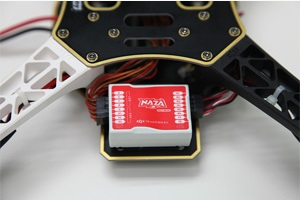
\includegraphics[width = 0.6\textwidth]{Bilder/NAZA_M-lite}
      \par\end{centering}
      \caption[Flightcontroller DJI NAZA-M lite]{Flightcontroller DJI NAZA-M lite\cite{NAZA_M-lite}}
      \label{NAZA_M-lite}
    \end{figure}

    \subsubsection{WLAN}
    Das WLAN-Modul RN171, welches von Microchip verkauft wird, bietet die Schnittstelle zwischen Server und Hexacopter. Die Daten können entweder vom Server gesendet
    und vom PIC empfangen werden oder umgekehrt.
    Das WLAM-Modul wird mit einer UART-Schnittstelle betrieben. Für eine Kommunikation sind also nur 2 Leitungen notwendig.
    Es bietet die Möglichkeit über eine Anwendung wie TeraTerm oder HTerm eingestellt zu werden, zusätzlich wird aber auch ein Webinterface angeboten, dieses muss jedoch zuvor
    aktiviert werden.

    \begin{figure}[tbh]
      \begin{centering}
        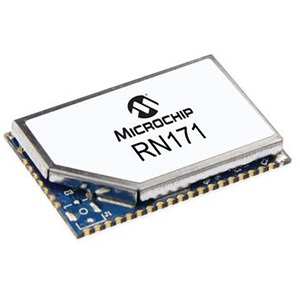
\includegraphics[width = 0.5\textwidth]{Bilder/RN171}
      \par\end{centering}
      \caption[WLAN-Modul RN171]{WLAN-Modul RN171\cite{RN171}}
      \label{RN171}
    \end{figure}

    Die Datenübertragung gestaltet sich dabei für den Nutzer sehr unproblematisch. Einerseits sind konfigurierbare Pins vorhanden um die Verbindung zu steuern und zu überwachen,
    andererseits braucht man sich nicht mehr um das Verpacken der Datenpakete kümmern.

%%%%%%%%%%%%%%%%%%%%%%%%%%%%%%%%%%%%%%%%%%%%%%%%%%%%%%%%%%%%%%%%%%%%%%%%%%%%%%%
\section{Blockschaltbild}
Die einzelnen Komponenten werden über den Mikrocontroller vereint. Sämtliche Berechnungen und Auswertung finden auf diesem statt und werden über diesen ausgegeben \bzw
weitergeleitet. Der Flightcontroller NAZA-M lite wird an die A, E, R und T Pins angeschlossen.
\begin{figure}[H]
  \begin{centering}
    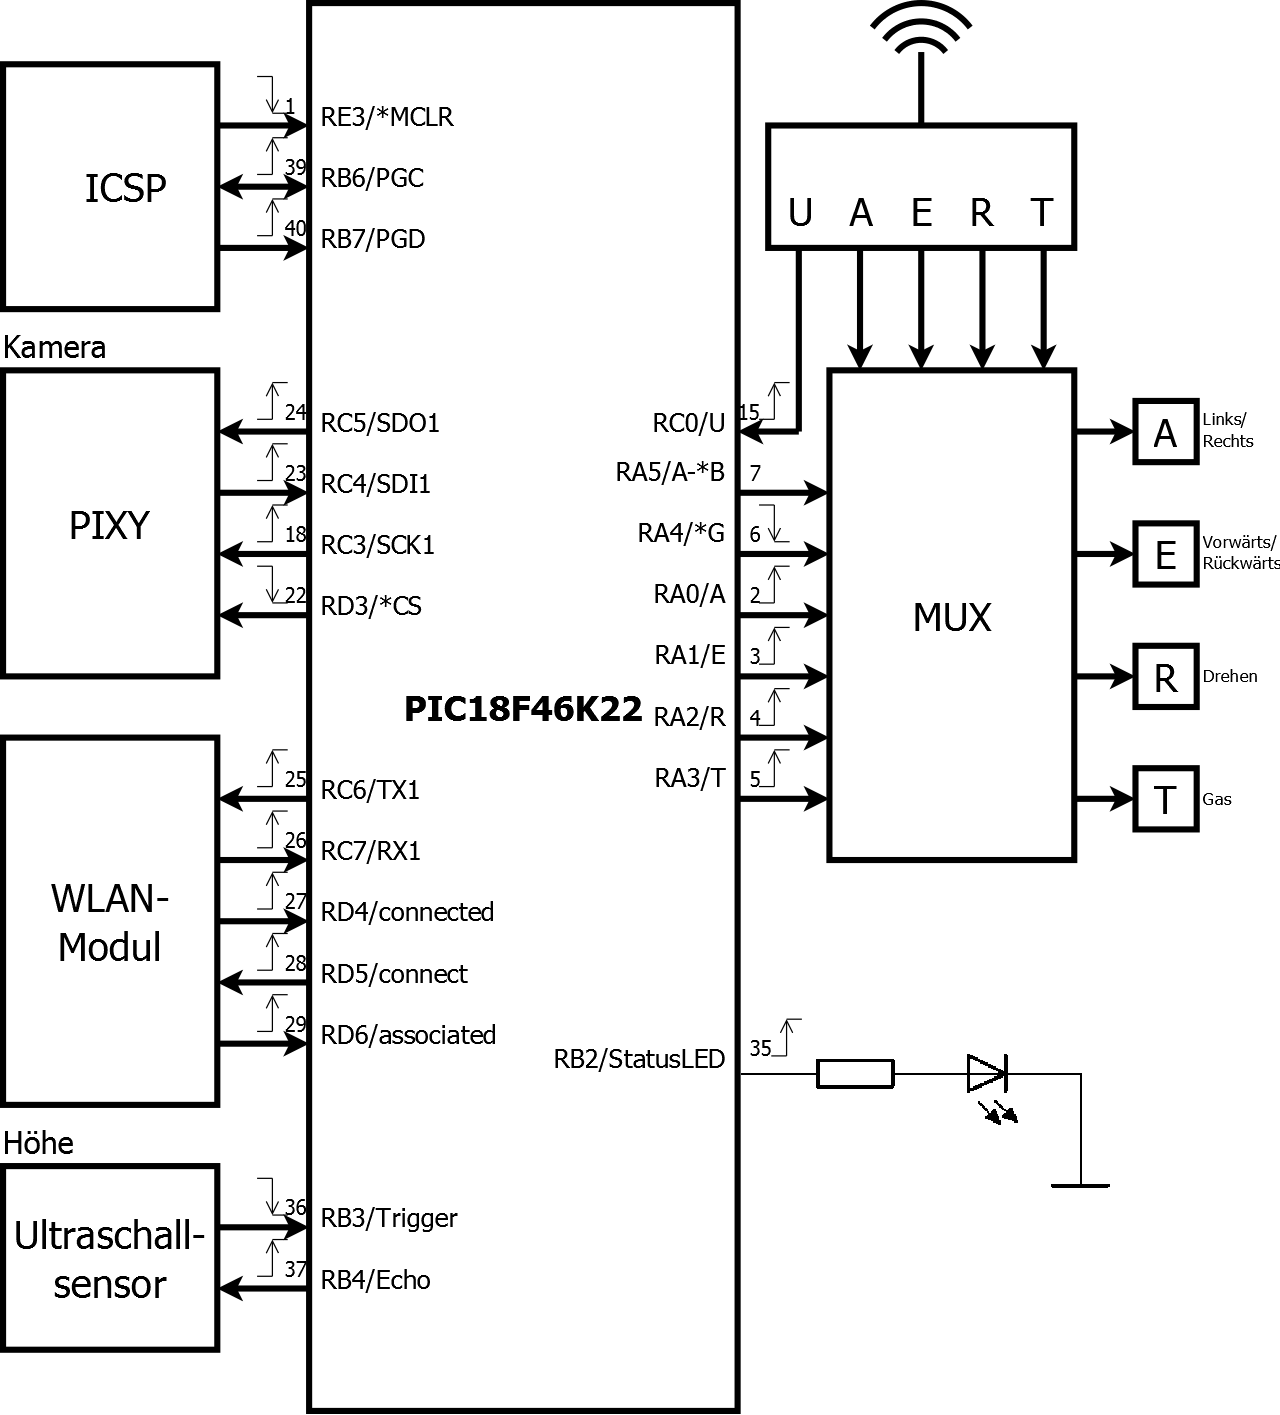
\includegraphics[width = 1\textwidth]{Bilder/Blockschaltbild}
  \par\end{centering}
  \caption{Blockschaltbild der Hauptplatine}
  \label{Blockschaltbild}
\end{figure}

  \subsection{Hauptplatine}
  Die Hauptplatine dient als zentrales Kommunikationselement. Auf ihr befindet sich der PIC welcher für sämtliche Berechnungen und Auswertungen zuständig ist.
  Um ein ausreichendes Maß an Kommunikationsfähigkeit zu ermöglichen, befinden sich auf ihr folgende Anschlüsse:
  \begin{itemize}
    \item $+\SI{5}{\volt}$ Spannungsversorgung
    \item Eingänge des Fernsteuerungsempfängers (5 Pins)
    \item Ausgänge zum Flightcontroller (4 Pins)
    \item Anschluss für den Ultraschallsensor
    \item Anschluss für die PIXY CMUcam5
    \item Anschluss für das WLAN-Modul
  \end{itemize}

    \subsubsection{Technische Planung}
    Das Hauptkriterium für die Hauptplatine war es alle notwendigen Komponenten für einen autonomen Flug zu enthalten. Wichtig waren hier vor allem die Kamera,
    der Ultraschallsensor sowie die Möglichkeit auf einen manuellen Flug zu wechseln.

    \subsubsection{Umsetzung}
    Für die Umsetzung wurden die einzelnen Komponenten entsprechend ihrer Funktion im Schalplan verbunden und aus diesem ein Platinen-Layout erstellt.
    Das Platinen-Layout wurde schließlich mit einem Fräsplotter auf das Rohmaterial übertragen.

    \begin{figure}[tbh]
      \begin{centering}
        \subfigure[Oberseite]{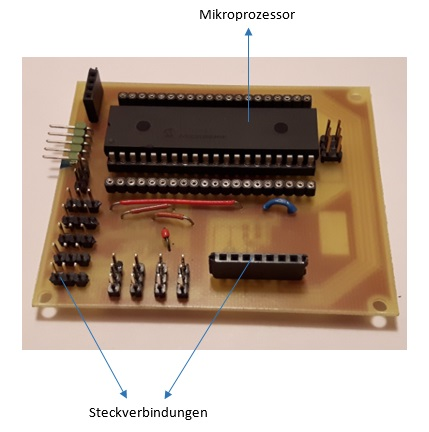
\includegraphics[width = 0.49\textwidth]{Bilder/HP_top}}
        \subfigure[Unterseite]{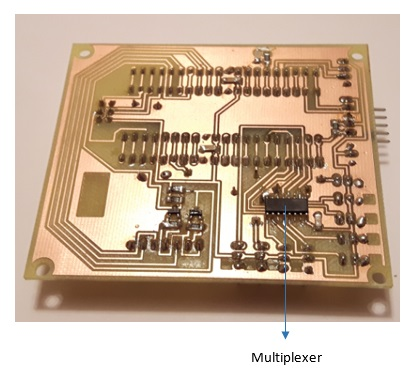
\includegraphics[width = 0.49\textwidth]{Bilder/HP_bot}}
      \par\end{centering}
      \caption{Die bestückte Hauptplatine}
      \label{Hauptplatine}
    \end{figure}

    \subsubsection{Herausforderungen und Lösungen}
    Eine Herausforderung stellte die geringe Deckkraft des schwarzen Toners beim ätzen der Platine dar. Durch zu wenig Toner auf der Belichtungsvorlage sind
    angeätzte Masseflächen entstanden. Um dennoch eine ordentliche Platine zu haben wurde diese schließlich gefräst. Dies hat auch viel Arbeit beim Bohren der
    Löcher erspart.

  \subsection{WLAN-Modul}
  Das WLAN-Modul dient als Schnittstelle zwischen Hauptplatine und Server. Auf dieser Platine befinden sich das WLAN-Modul RN171 sowie ein Spannungsregler und Level-Shifter
  um eine Kompatibilität mit den anderen Komponenten zu gewährleisten.

    \subsubsection{Technische Planung}
    In der Planung war die Versorgungsspannung des WLAN-Modul das Hauptaugenmerk. Für den Betrieb sind $\SI{3.3}{\volt}$ notwendig, die Versorgungsspannungstoleranz
    des WLAN-Moduls ist nicht groß genug, um dieses mit $\SI{5}{\volt}$ versorgen zu können.
    Aufgrund der fehlenden Toleranz müssen alle Leitungen die zur Kommunikation dienen entweder auf $\SI{5}{\volt}$ angehoben oder auf $\SI{3.3}{\volt}$ abgesenkt werden,
    andernfalls kann es zu Datenverlust oder sogar einer Beschädigung eines Moduls kommen.

    \subsubsection{Umsetzung}
    Auch für diese Platine wurde ein Schaltplan und Layout erstellt. Anschließend wurde das Layout wieder mit einem Fräsplotter auf das Rohmaterial übertragen.

    \begin{figure}[tbh]
      \begin{centering}
        \subfigure[Oberseite]{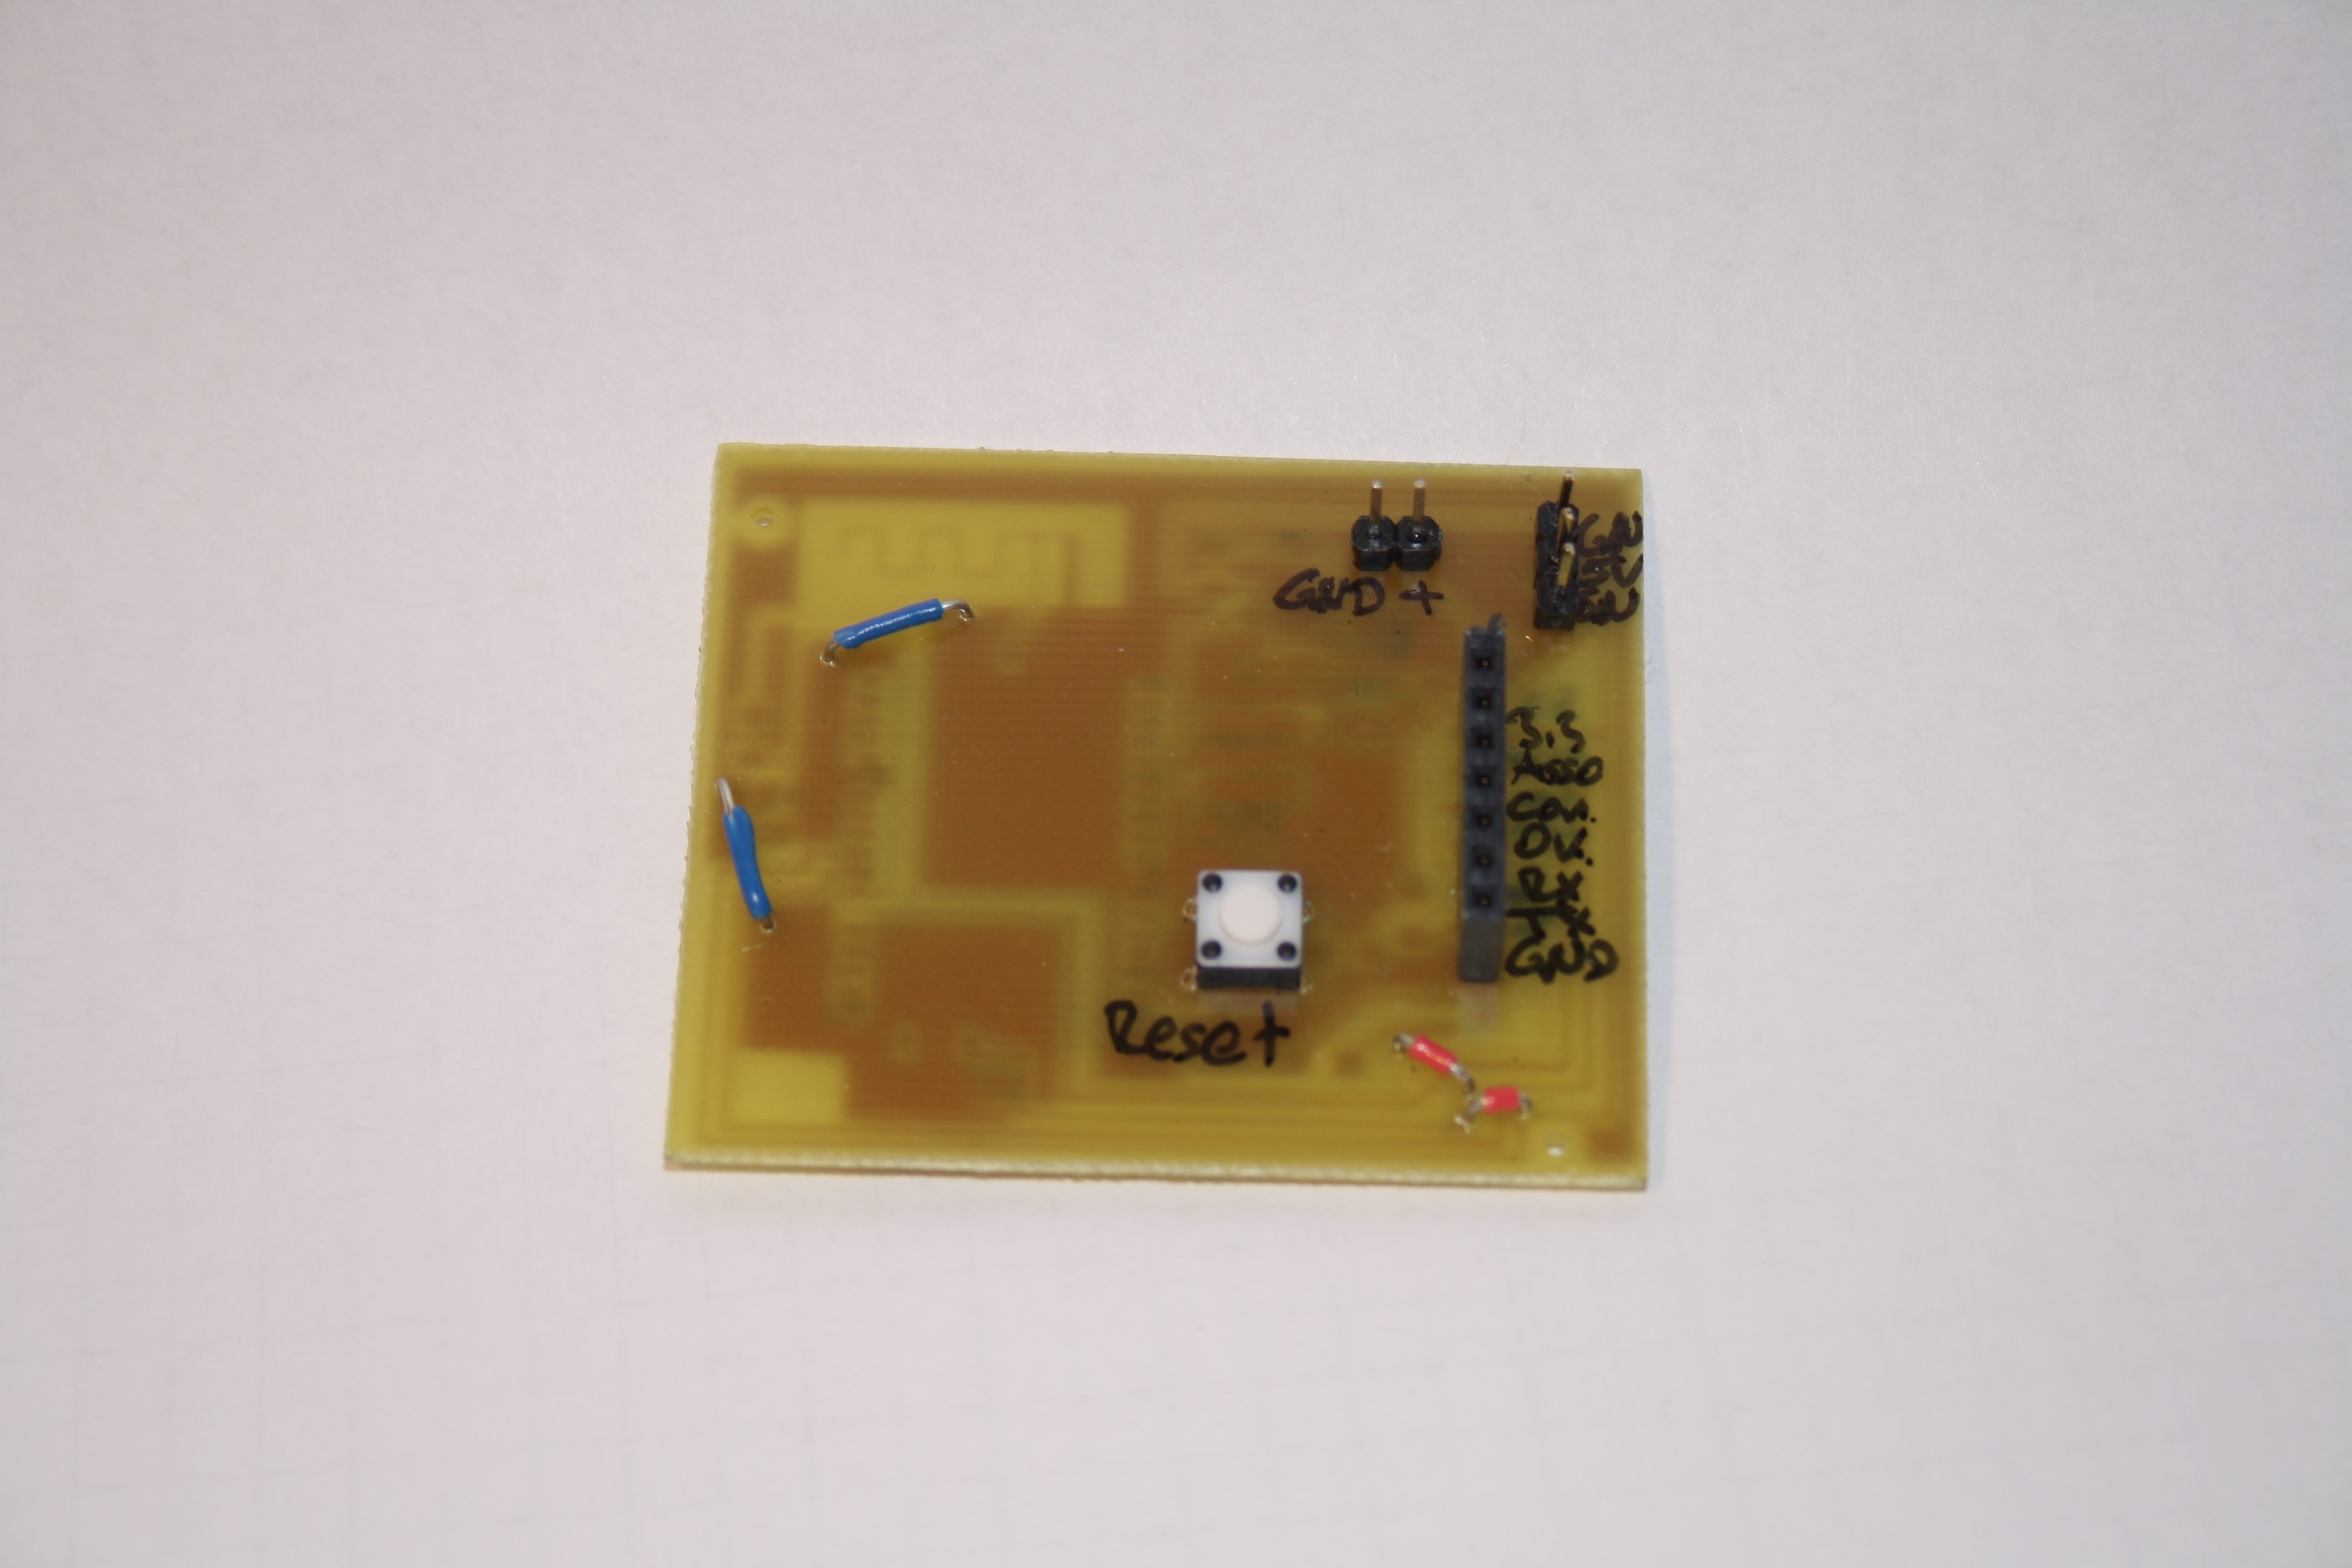
\includegraphics[width = 0.49\textwidth]{Bilder/WLAN_top}}
        \subfigure[Unterseite]{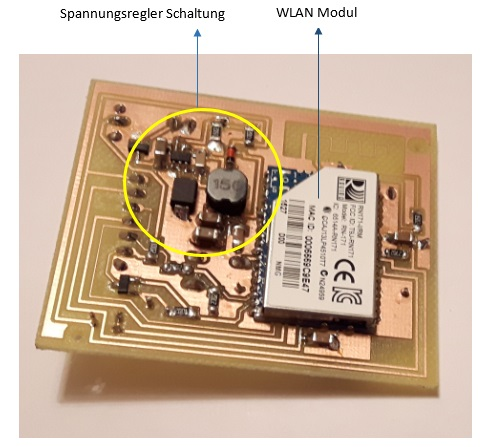
\includegraphics[width = 0.49\textwidth]{Bilder/WLAN_bot}}
      \par\end{centering}
      \caption{Die bestückte WLAN-Platine}
      \label{WLAN-Platine}
    \end{figure}

    %\begin{figure}
    %  \centering
    %  \begin{subfigure}[h]{0.49\textwidth}
    %    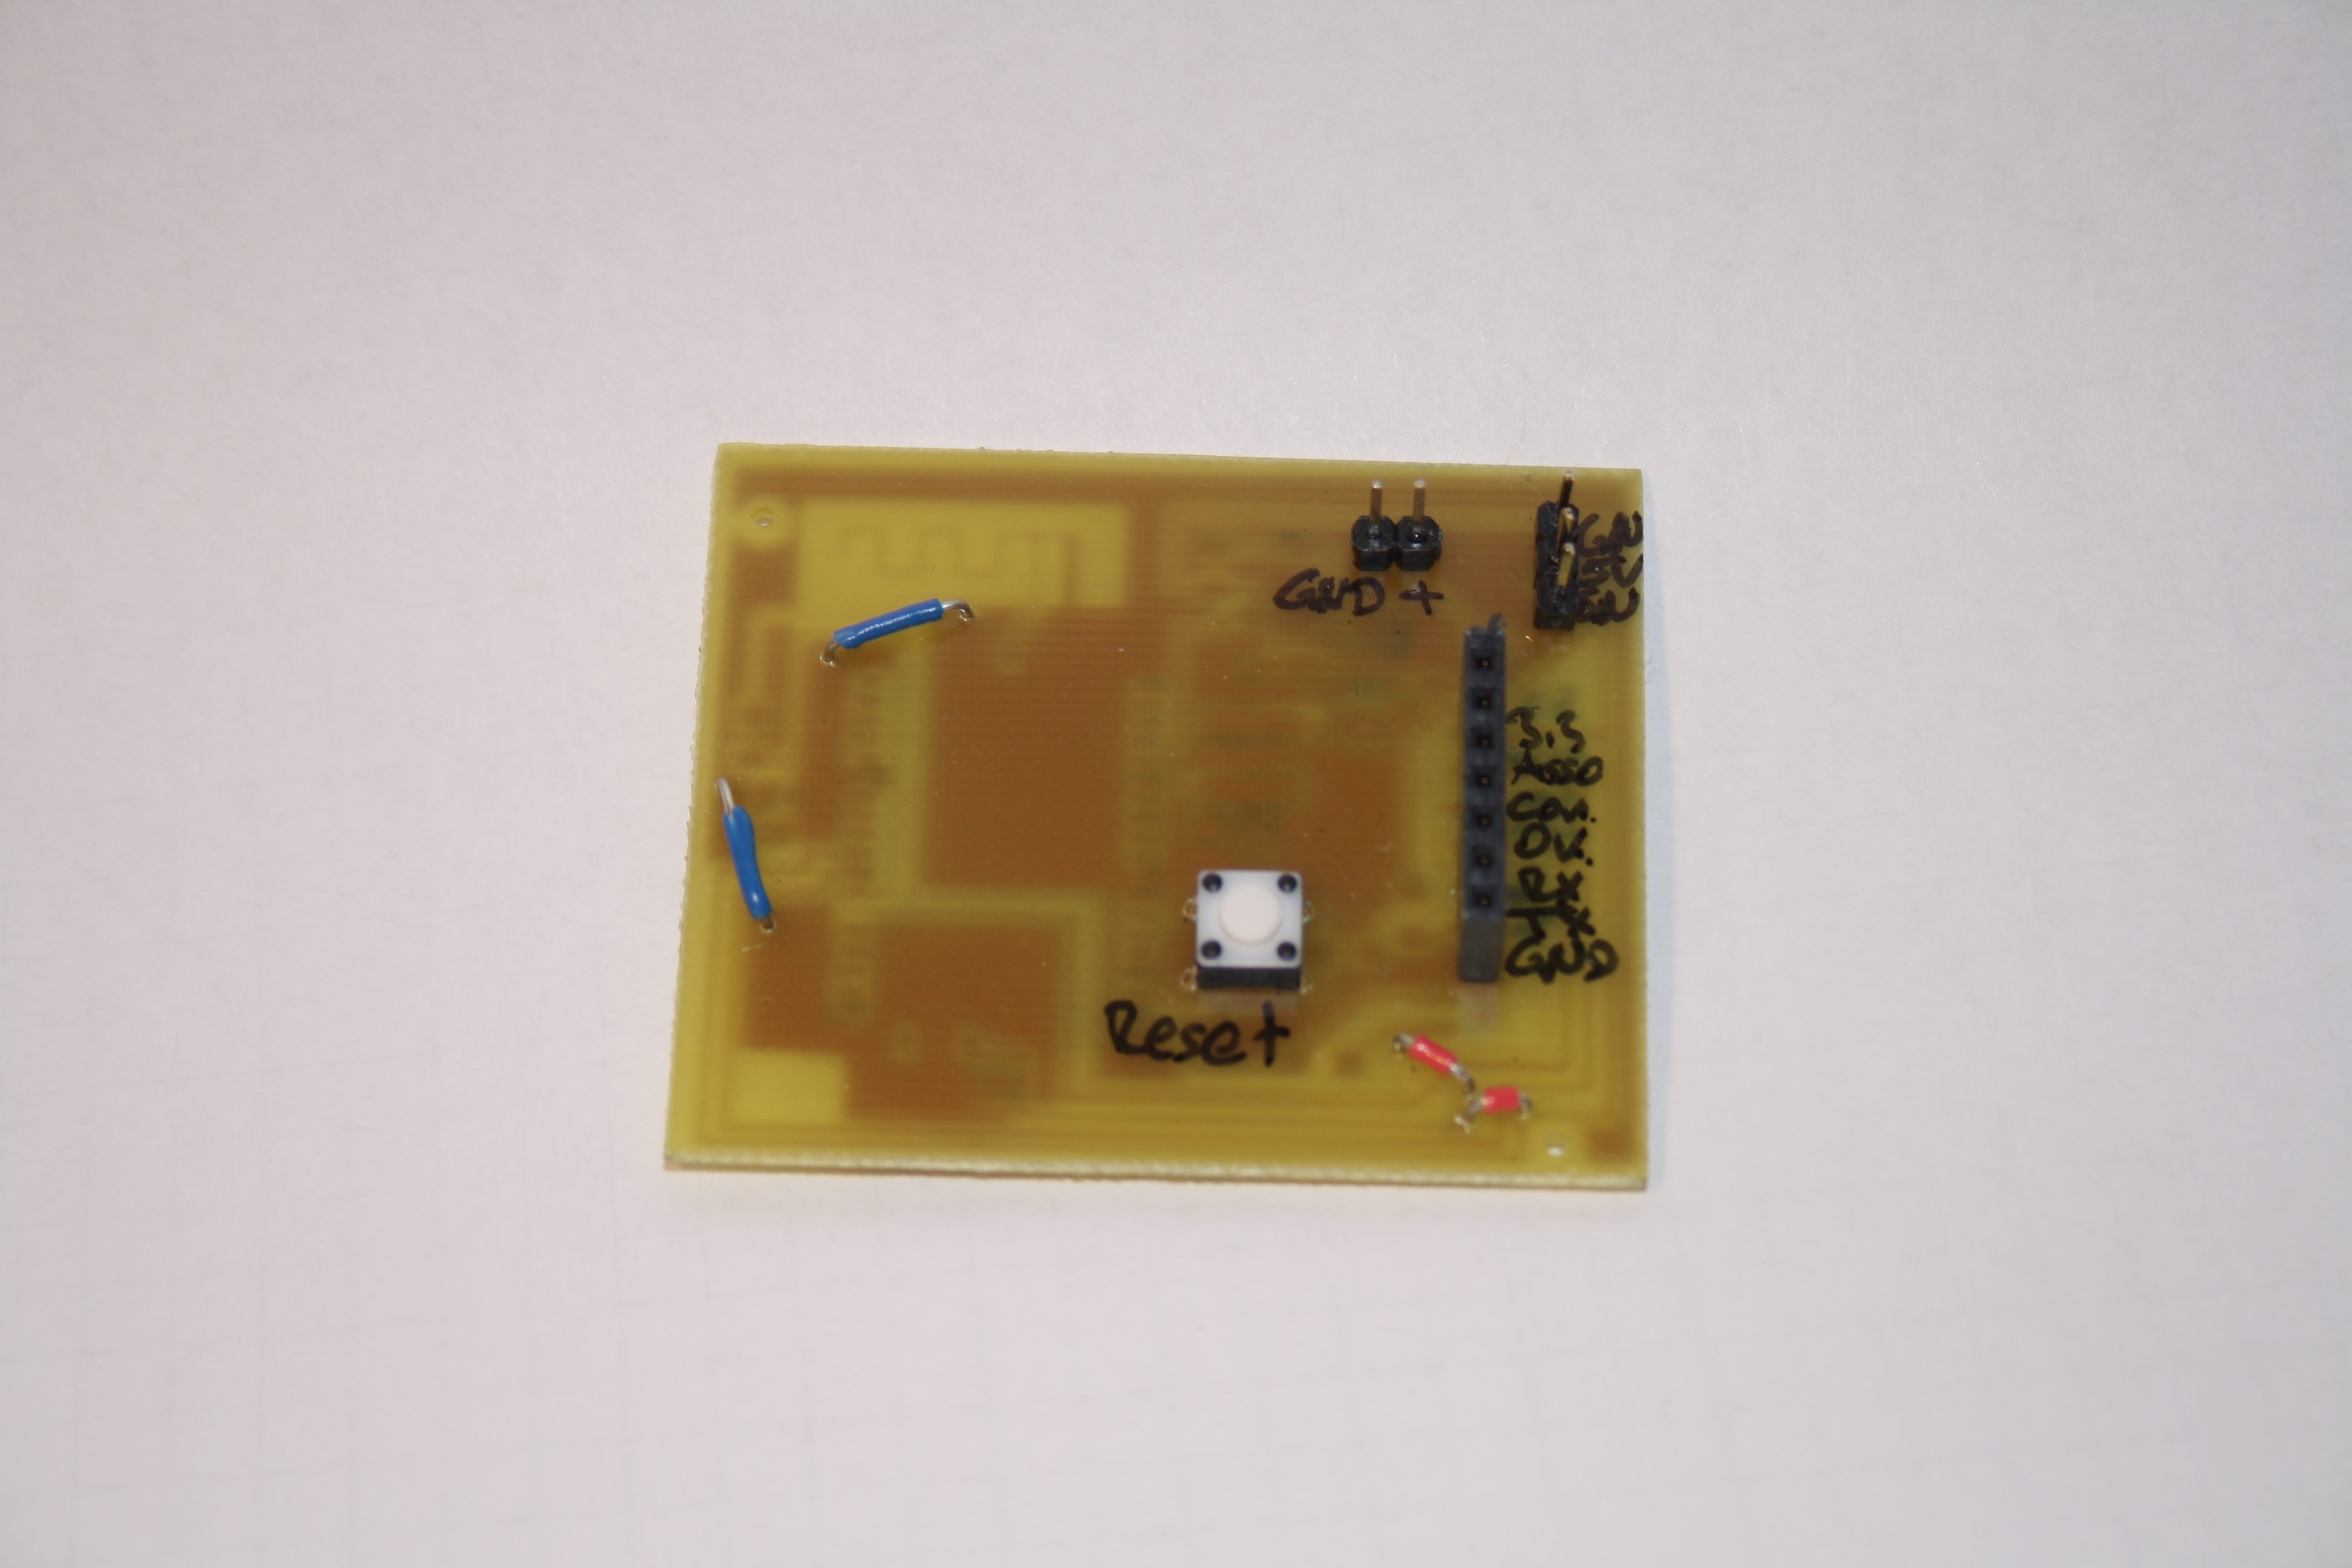
\includegraphics[width = \textwidth]{Bilder/WLAN_top}
    %    \caption{Oberseite}
    %  \end{subfigure}
    %  \begin{subfigure}[h]{0.49\textwidth}
    %    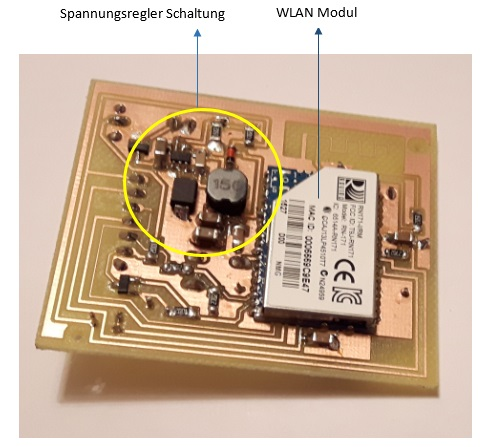
\includegraphics[width = \textwidth]{Bilder/WLAN_bot}
    %    \caption{Unterseite}
    %  \end{subfigure}
    %  \caption{Die bestückte WLAN-Platine}
    %  \label{WLAN-Platine}
    %\end{figure}

    \subsubsection{Herausforderungen und Lösungen}
    Um eine funktionierende Kommunikation sicher stellen zu können, wurden mehrere Level-Shifter in Richtung des Mikroprozessors sowie Spannungsteiler in Richtung des WLAN-Moduls
    integriert. Diese Maßnahmen sorgen dafür, dass weder das WLAN-Modul beschädigt wird, noch Daten verloren gehen.
    Bei der Platinen-Fertigung wurde aufgrund der schlechten Deckkraft abermals auf den Fräsplotter zurückgegriffen.


% !TEX root = diplomarbeit.tex
\chapter{Firmware}
\renewcommand{\kapitelautor}{Autor: Christina Bornberg, Lucas Ullrich}

%%%%%%%%%%%%%%%%%%%%%%%%%%%%%%%%%%%%%%%%%%%%%%%%%%%%%%%%%%%%%%%%%%%%%%%%%%%%%%%
\section{Allgemeine technische Planung}

  \subsection{Konvention}
  In der Arbeit wird folgende Konvention festgelegt. Die z-Achse ist die Höhe, die y-Achse ist vorwärts und rückwärts und die x-Achse ist seitwärts.

  % BILD %

  \subsection{Tischplan}
  Das Konzept Tischplan beschreibt den Aufbau des Restaurants, also welche Komponenten benötigt werden und wo diese platziert sind.
  Um eine vorgegeben Route fliegen zu können muss dem Multicopter ein Routenplan bereitgestellt werden, in welchem die einzelnen Markierungspunkte enthalten sind, die der Multicopter auf seinem Weg zum Tisch überfliegt.

  Für den Tischplan wird die symbolische Positionierung genutzt. Er besteht aus folgenden Komponenten:

  \subsection*{Küche}
  Die Küche beschreibt den Bereich, in dem der Kellner interagiert. Hier befindet sich die Base, eine Plattform, die mit einem Farbcode ausgestattet ist. Auf ihr steht der Hexacopter und wartet auf die Beladung des auszuliefernden Cupcakes und den Befehl, loszufliegen.
  Das Admin Interface und der Server stehen ebenfalls in der Küche, über diese Komponenten bekommt der Hexacopter Befehle. Die Routen zu jedem Tisch sind im Admin Interface hinterlegt.

  \subsection*{Weg}
  Der Weg besteht, aus sich abwechselnden zweifarbigen Codes. Die Bereiche zwischen Tischen und Kreuzungen, werden als Wegabschnitt bezeichnet. Die ColorCodes müssen von jedem Restaurant eigenständig eingescannt und die Routen zum jeweiligen Tisch in das Admin Interface eingetragen werden.

  \subsection*{Tisch}
  Auf einem Tisch befindet sich, wie in der Küche, eine Plattform, die mit einem Farbcode versehen ist. Hier landet der Hexacopter, wartet 30 Sekunden lang und fliegt danach den Weg zurück zu seiner Base. In den 30 Sekunden soll der Cupcake entnommen werden. Weiters befindet sich ein iPad auf jedem Tisch. Durch dieses erhält jeder Tisch seine eigene ID und die dazugehörige Route. Bestellungen können somit einem Tisch zugewiesen werden.
  Die Tische können wie in jedem normalen Restaurant beliebig platziert werden, da der Hexacopter durch die Rotation der Farbobjekte auch Kurven fliegen kann. Dabei darf ein Teil des Tisches nicht besetzt sein, da die Drohne nicht über Menschen fliegen soll.

  % Bild vom Ablauf %%%%%%%%%%%%%%%%%%%%%%%%%%%%%%%%

  \subsection{Flussdiagramme}
  Für einen besseren Überblick über die einzelnen Programme und deren geforderten Funktionen wurden einzelne Flussdiagramme des gesamten Prozesses erstellt.
  Diese dienen nachfolgend als Orientierung beim Programmieren der einzelnen Funktionen.

  \begin{figure}[tbh]
    \begin{centering}
      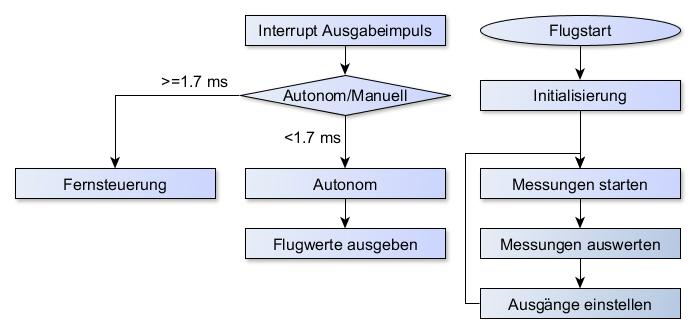
\includegraphics[width = \textwidth]{Bilder/Flussdiagramm}
    \par\end{centering}
    \caption{Flussdiagramm des Gesamtablaufs}
    \label{Flussdiragramm}
  \end{figure}

  Für die weiteren Programmteile wurden jeweils noch detailliertere Flussdiagramme erstellt.

%%%%%%%%%%%%%%%%%%%%%%%%%%%%%%%%%%%%%%%%%%%%%%%%%%%%%%%%%%%%%%%%%%%%%%%%%%%%%%%
\section{Navigation}

  \subsection{Technische Planung}

    \subsection*{Frames}
    Ein Frame entsteht bei jeder Messung der Pixy CMUcam5. Der Frame hat eine Breite von 319 und eine Höhe von 199 Pixel. Die Koordinate (0/0) befindet sich in der linken oberen Ecke.

    Bild 1 beschreibt den alten Frame, Bild 2 den aktuellen. Die Position des Objektes, beschreibt die zentralen x und y Positionen im Frame. Die Differenz entsteht aus den unterschiedlichen Positionen des Objektes im alten und neuem Frame. Das Objekt soll in den Bereich zwischen X\_MIN und X\_MAX, beziehungsweise Y\_MIN und Y\_MAX gelangen.

    % BILD VON LUCAS %

    \subsection*{Aileron}
    Anhand des aktuell getrackte Colorcodes wird die seitliche Position korrigiert. Solange sich der Hexacopter nicht im angegeben Bereich befindet, wird die Fluggeschwindigkeit in die jeweilige Richtung erhöht.

    \subsection*{Elevator}
    Durch den getrackten Colorcode, wird die Vorwärts- beziehungsweise Rückwärtsbewegung eingestellt. Die Position des Markers soll sich, wie bei der Bewegung nach Links und Rechts, in einem vorgegebenen Bereich befinden. 
    Das Kamerasystem trackt den ersten Marker, bis er sich im richtigen Bereich befindet und der zweite Marker erkannt wird, dieser wird ebenfalls verfolgt, danach kommt der dritte. Diese Routine läuft, bis der letzte Colorcode erreicht ist. Im Idealfall muss die Rückwärtsbewegung während des Fluges gar nicht durchgeführt werden. Die Rückwärtsbewegung findet ihre Anwendung nur, wenn der Hexacopter beim letzten Farbcode angekommen ist und über sein Ziel hinausfliegt, oder, wenn kein nächster Farbcode gefunden wird. Welcher Marker der Zielmarker ist, kann durch die Größe des Arrays, in dem die Marker gespeichert werden, herausgefunden werden. Dieses wird mit den Daten, die im Admin-Interface hinterlegt sind und im Endeffekt vom Wlan-Modul empfangen werden, befüllt.

    \subsection*{Rudder}
    Mithilfe der Rudder Funktion muss der Winkel auf die aktuelle Positionsmarkierung ausgerichtet werden. Dabei ist eine Ungenauigkeit von 5 Grad in beide Richtungen erlaubt.

    Für die Rotation werden die Grundlagen negativer binärer Zahlen benötigt.

    \begin{itemize}
    \item \textbf{Binäre Zahlen ohne Vorzeichen}\\
    0000 0000 = 0, 1111 1111 = 255
    \item \textbf{Binäre Zahlen mit Vorzeichen} - Ein Bit wird für das Vorzeichen verwendet. \\
    0000 0001 = 1 -> 1000 0001 = -1, \\
    0111 1111 = 127 -> 1111 1111 = -127
    \item \textbf{Einerkomplement} - Beim Invertieren aller Bits entsteht eine negative Zahl \\
    0000 0000 = "+0" -> 1111 1111 = "-0" \\
    0111 1111 = 127 -> 1000 0000 = -127
    \item \textbf{Zweierkomplement}\\
    0000 0001 = 1 -> 1111 1111 = -1 \\
    0000 0010 = 2 -> 1111 1110 = -2 \\
    0111 1111 = 127 -> 1000 0001 = -127
    \item \textbf{Bilden des Zweierkomplements}\\
    \textbf{Beispiel:} 0111 1111 = 127 \\
    Die binäre Zahl wird invertiert (1000 0000) und mit 1 addiert. \\
    Das Ergebins lautet: 1000 0001 = -127 \\
    \textbf{Beispiel:} 1001 1000 = -104 \\
    Die binäre Zahl wird invertiert (0110 0111) und mit 1 addiert. \\
    Das Ergebnis lautet: 0110 1000 = 104 \\
    \end{itemize}

    % Bild von Rotation %

    \subsection*{Throttle}
    Über den Ultraschallsensor erfährt der Hexacopter, wie hoch er fliegt. Beim Erreichen der maximalen Flughöhe, wird seine Antriebskraft gesenkt. Dadurch korrigiert er seine Höhe bei jedem Aufruf der Funktion und eine Änderung des Gewichts, kann ausgeglichen werden. Der entnommene Cupcake und die damit verbundene Gewichtsveränderung stellt daher kein Problem dar.

  \subsection{Umsetzung}

    \subsubsection{Vergleichen der Frames}
    Für den Vergleich des aktuellen Frames mit dem letzten Frame, werden zwei \glslink{Struktur}{Strukturen} verwendet, die über folgende Mitglieder verfügt. \cite{Structs}
    \begin{itemize}
      \item \textbf{num} ist die ID des getrackten Colorcodes, er besteht aus einer zweistelligen Zahl.
      \item \textbf{pos\_x} ist die X-Position des Colorcodes. Der Wert bezieht sich auf das Zentrum des Objektes.
      \item \textbf{pos\_y} ist die Y-Position des Colorcodes. Der Wert bezieht sich auf das Zentrum des Objektes.
      \item \textbf{height} ist die, vom Ultraschall übergebene Höhe.
      \item \textbf{angle} ist die Rotation des Colorcodes. Da er zweifarbig ist, kann die PIXY CMUcam5 die Rotation des Objektes feststellen.
    \end{itemize}

    Zuerst wird die ID des Colorcodes verglichen, um herauszufinden, ob das Farbobjekt das selbe ist, wie im letzten Frame.
    Sollte dies der Fall sein, werden die Koordinaten x und y und die Rotation mit den Werten der älteren Struktur verglichen und in einer weiteren Strunktur gespeichert. Dieses wird bei den folgenden Funktionen verwendet, um anhand der Änderung zwischen zwei Frames zu überprüfen, ob der Hexacopter die richtige Geschwindigkeit hat.

    \subsubsection{Aileron, Elevator und Rudder anhand der Kameradaten}
    Durch die PIXY CMUcam5 kann die Position des Hexacopters, relativ zu einem Colorcode, festgestellt werden. Gegebenenfalls werden anschließend die Flugparameter verändert.

    \begin{figure} [tbh]
      \begin{centering}
        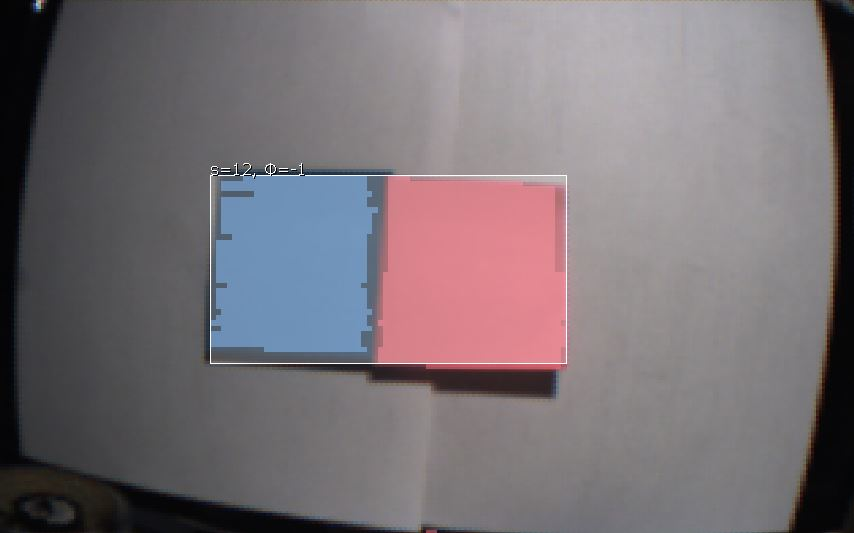
\includegraphics[width = \textwidth]{Bilder/Farbcode_erkannt}
      \par\end{centering}
      \caption{Ein erkannter Farbcode}
      \label{Farbcode_erkannt}
    \end{figure}
    Die Position wird anhand solcher Farbcodes erkannt, im Tischkonzept ist hinterlegt in welcher Reihenfolge der Hexacopter die Farbcodes suchen muss.
    Er fliegt anschließend so lange, bis er über dem aktuellen Farbcode ist, dieser also mittig im Bild ist und sucht darauf den nächsten.

    \subsubsection{Überprüfen von Aileron}
    Beim Vergleichen von Aileron wird die Veränderung an der x-Achse überprüft.

    Durch diese Funktion soll der Hexacopter mithilfe der Pixy-Daten, den Colorcode in der Mitte des Frames plazieren. An der x-Achse sind Werte zwischen 150 und 170 optimal. Der übergebene Wert ist dabei der Mittelpunkt des Colorcodes.
    Sollte die Pixycam keinen Wert in diesem Bereich erfassen, kann sie durch eine weitere Funktion namens ActAileron, welche die Änderungsrate an den Flightcontroller weitergibt, die Position an der x-Achse korrigieren.
    Um herauszufinden, ob der Mittelpunkt unter oder über dem optimalen Wert liegt, also der Hexacopter zu weit links oder rechts vom Objekt fliegt, gibt es für beide Fälle eine Abfrage.
    Um den Aileron Wert entgültig zu setzen, müssen nach der Überprüfung, ob der übergebene Wert an der x-Achse 170 überschreitet beziehungsweise 150 unterschreitet, folgende Zustände kontrolliert werden.
    Zunächst muss der Hexacopter über die Pixycam herausfinden, ob er sich bereits in die richtige Richtung bewegt. Dafür werden die beiden Frames miteinander verglichen. Wenn der Wert zu hoch ist, muss der x-Wert im alten Frame größer als im neuen sein. Sollte er zu niedrig sein, muss der Wert im neuen Frame höher sein.
    Anderenfalls fliegt der Hexacopter auf die falsche Seite. Die Firmware reagiert darauf mit der Änderung der Pulszeit am Aileron-Pin.
    Bei der Bewegung in die richtige Richtung wird der Wert so lange in diese gesteuert, bis sich die Geschwindigkeit, gemessen in den veränderten Pixel zwischen zwei Frames, zwischen zwei konstanten Werten befindet.

    \subsubsection{Überprüfen von Elevator}
    Elevator, die Bewegung an der y-Achse, also die Bewegung nach vorne und nach hinten, funktioniert nach dem selben Prinzip wie Aileron.

    Zuerst wird kontrolliert, ob sich der Farbcode im gewünschten Bereich befindet, in diesem Fall zwischen 90 und 110.
    Sollte der Mittelpunkt an der y-Achse nicht in diesem Bereich liegen, fliegt der Hexacopter nach vorne beziehungsweise zurück.
    Da die Route aus mehreren Farbcodes besteht, richtet sich der Hexacopter, sobald der Colorcode im Bereich zwischen 90 und 100 liegt, nach dem Objekt, das sich am nächsten zum Nullpunkt der y-Achse befindet. Somit probiert er die Position zentriert über dem Farbobjekt zu optimieren, bis er das nächste Farbobjekt erkennt und trackt. Das alte Objekt ist nun unwichtig, der Hexacopter bezieht sich auf das vordere Farbobjekt.

    Wie bei der Überprüfung von Aileron, gibt es auch hier zwei konstante Werte, zwischen denen sich die Geschwindigkeit befinden soll, solange die Position optimiert wird.

    \subsubsection{Überprüfen von Rudder}
    Rudder beschreibt die Rotation um seine eigene Hochachse. Dafür wird zunächst unterschieden, ob sich der Hexacopter am Hin- oder Rückflug befindet, da die Rotation der Colorcodes beim Rückflug um 180 Grad gedreht werden muss.

    Die optimale Rotation befindet sich beim Hinflug zwischen -5 und 5 Grad.
    Bei einem zu niedrigen oder zu hohen Wert wird kontrolliert, ob sich der Hexacopter bereits in die richtige Richtung dreht.
    Sollte dies nicht der Fall sein, wird die Änderungsrate an die dazugehörige Funktion geschickt, die dem Flightcontroller die Information zur Beschleunigung gibt.
    Ansonsten wird die Veränderung der Pixel zweier Frames verglichen, wenn sie sich im gewünschten Bereich befindet, wird der Wert nicht geändert, bei einem zu hohen Wert, wird die Rotationsgeschwindigkeit gesenkt, ansonsten erhöht.

    Beim Rückflug soll die Rotation des Colorcodes größer als 175 oder kleiner als -175 sein.

    \subsubsection{Throttle anhand des Ultraschallsensors}
    Der Hexacopter steht auf einer Landeplattform in seiner Base. Unter ihm ist ein Farbcode, den er so lange fokusiert, bis er den nächsten Farbcode trackt. Den zweiten Farbcode kann er erst scannen, wenn er hoch genug fliegt um an der Tischkante vorbei, den nächsten Farbcode zu scannen.

    Beim Starten fliegt er vertikal nach oben, bis er den zweiten Farbcode erkennt. Um beim Start nicht abzudriften, beschleunigt er, solange er sich unter einer Höhe von $\SI{50}{\centi\metre}$ befindet, mit einer hohen Änderungsrate. Ab dieser Höhe beschleunigt er mit einer geringeren Erhöhung der Änderungsrate, bis er die $\SI{80}{\centi\metre}$-Grenze erreicht hat.
    zwischen $\SI{80}{\centi\metre}$ und $\SI{120}{\centi\metre}$ bleibt die Beschleunigung gleich, das führt jedoch dazu, dass der Hexacopter den oberen Rand von $\SI{120}{\centi\metre}$ erreichen wird, da er bis jetzt nicht gebremst wird. Sobald er über $\SI{120}{\centi\metre}$ kommt, wird die Beschleunigung reduziert. Der Hexacopter pendelt sich zwischen $\SI{80}{\centi\metre}$ und $\SI{120}{\centi\metre}$ ein.

    Nun wird berechnet, ob er sich noch über dem Tisch oder schon über dem Boden befindet. Dies stellt er fest, wenn zwei hintereinanderliegende Messungen einen Höhenunterschied von $\SI{50}{\centi\metre}$ aufweisen. Die zweite Messung ist erforderlich, um mögliche Fehlmessungen auszuschließen.

    Wenn er nun über dem Boden fliegt, beträgt seine minimale Höhe $\SI{180}{\centi\metre}$ und seine maximale Höhe $\SI{220}{\centi\metre}$.
    Der Hexacopter beschleunigt nach dem selben Prinzip, wie über einem Tisch. Unter $\SI{100}{\centi\metre}$ ändert er seine Beschleunigung mit einem hohen Wert. Bis $\SI{180}{\centi\metre}$ beschleunigt er mit einer niedrigeren Änderungsrate. Sollte der Hexacopter über $\SI{220}{\centi\metre}$ fliegen, wird die Beschleunigung durch eine negative Änderungsrate gesenkt.

    Der Hexacopter fliegt mit diesen Werten, bis er den vorletzten Farbcode erreicht hat. Da die Farbcodes in einem Array abgespeichert werden, ist die Anzahl der darin gespeicherten Farbcodes bekannt.

    Beim letzten Farbcode angekommen, also dem am Tisch liegenden Farbcode, wird ebenfalls wieder durch die Kontrolle von zwei Werten, die sich um $\SI{50}{\centi\metre}$ von der vorigen Messung unterscheiden müssen, analysiert, wann sich der Hexacopter über dem Tisch befindet. Sobald dies der Fall ist, landet er, indem er die Beschleunigung mit einer negativen Änderungsrate verlangsamt. Dabei muss er sich, zwischen einer vom System vorgegebenen Mindest- und Maximalgeschwindigkeit, befinden.

    Nach der Landung wird die Routeninformation umgekehrt, der erste Colorcode wird zum letzten, der zweite zum vorletzten und so weiter. Außerdem muss die Rotation der Farbcodes beim Rückflug um 180 Grad gedreht sein, dafür wird die Richtung als Rückflug abgespeichert. Sollte sich der Hexacopter wieder in der Base befinden, wird die Variable wieder als Hinflug gespeichert.

    Damit genügend Zeit für das herunternehmen des Cupcakes ist, verweilt der Hexacopter eine halbe Minute am Tisch, bevor er seinen Rückflug antritt.

    \subsubsection{Speichern der alten Daten}
    Die alten Daten werden gespeichert, um die Differenzen von zwei Frames zu errechnen. Der Frame mit Index 0, ist der aktuelle Frame, der Frame mit dem Index 1, der alte. Bei jedem Durchlauf, werden die Werte aktualisiert.

    \subsubsection{Ausgabe der Steuersignal}
    Autor: Lucas Ullrich\\
    Nachdem die Steuersignale berechnet und korrigiert wurden, müssen diese an den Hexacopter ausgegeben werden. Dies muss periodisch alle $\SI{20}{\milli\second}$ geschehen.
    Der Flightcontroller erkennt jeweils die einzelnen Impulse und steuert die Rotoren entsprechend an.

    Diese Impulse werden interruptgesteuert ausgegeben, der Interrupt wird von dem Gear-Pin erzeugt, welcher gleichzeitig für den Flugmodus verantwortlich ist.

    \lstset{language = c}
    \begin{lstlisting}
interrupt void Isr() {
  if(CCP1IF == 1) {
    CCP1IF = 0;
    T1CONbits.TMR1ON = 0;
    SignalOut();
    NOP();
  }
  if(TMR3GIF == 1) {
    TMR3GIF = 0;
    ModeCheck();
    SignalOut();    /* initial call after remaining break to 20 ms
                     * starts with Aileron (needs to be set in last
                     * case statement, case 0) following delays will
                     * be processed by the previous routine */
    pulsecounter++;
  }
}

void SignalOut(void) {
  switch(pin_out) {
    case 'A': {
      A = 1;
      Delay(a_actors[0].aile);
      pin_out = 'E';
      break;
    }case 'E': {
      A = 0;
      E = 1;
      Delay(a_actors[0].elev);
      pin_out = 'T';
      break;
    }
    \end{lstlisting}
    Die weiteren Signale (Throttle und Rudder) werden auf die gleiche Weise ausgegeben.
    Die Delay-Funktion stellt die Compare-Einheit so ein, dass nach der gewünschten Pulsdauer des Ausgangs ein Interrupt hervorgerufen wird.

%%%%%%%%%%%%%%%%%%%%%%%%%%%%%%%%%%%%%%%%%%%%%%%%%%%%%%%%%%%%%%%%%%%%%%%%%%%%%%%
%\section{Objekterkennung}

  %\subsection{Technische Planung}

  %\subsection{Umsetzung}

  %\subsection{Herausforderungen und Lösungen}

%%%%%%%%%%%%%%%%%%%%%%%%%%%%%%%%%%%%%%%%%%%%%%%%%%%%%%%%%%%%%%%%%%%%%%%%%%%%%%%
\section{Sicherheit}

  \subsection{Technische Planung}

Sicherheitskonzepte

Beim Konzept Sicherheitsmaßnahmen geht es grundsätzlich um die Sicherheit von Mensch, Umgebung und dem Multicopter selbst. Hier werden mögliche Fehler mit Anlehnung an FMEA ("Fehlermöglichkeits- und -einflussanalyse" / "Auswirkungsanalyse") analysiert. Dieses Konzept ist ein rein schriftliches Konzept.

  \subsection{Umsetzung}

    Legende:
    \begin{itemize}
    \item A: Auftreten
    \item B: Bedeutung
    \item E: Entdeckung
    \item RPZ: Risiko-Prioritätszahl = A * B * E
    \end{itemize}

    Die Werte beziehen sich auf den Fehler, die obere Analyse beschreibt das Auftreten, die Bedeutung und die Entdeckung vor den Maßnahmen, die unteren nach den Maßnahmen.

%\begin{table}[H]
%\centering
\begin{longtable}{|p{0.4cm}|p{3.0cm}|p{3.1cm}|p{3.1cm}|p{0.4cm}|p{0.4cm}|p{0.4cm}|p{0.8cm}|}

\hline \#   & Bezeichnung                                                                                               & Fehler                                                                                                                & Beschreibung                                                                                                                    & A   & B   & E   & RPZ \\
 1          & Mensch in unmittelbarer Nähe                                                                              & Mensch wird verletzt, da Hexacopter nicht ausweicht                                                                   & Eine Person steht auf dem Weg und wird vom Hexacopter als Hindernis erkannt                                                     & 5   & 10  & 10  & 500 \\
\hline -    & Vermeidung                                                                                                & Maßnahme nach Eintritt                                                                                                & Mögliche Softwarelösung                                                                                                         & A   & B   & E   & RPZ \\
 -          & Wege absperren, Menschen darauf hinweisen, sich nicht in unmittelbarer Nähe des Hexacopters aufzuhalten.  & Hexacopter landet auf der Stelle um die Sicherheit der Person zu gewährleisten.                                       & Durch 2 Ultraschallsensoren, die vorne am Hexacopter angebracht sind, werden Menschen erkannt, er landet daraufhin.             & 2   & 10  & 5   & 100 \\\hline

\hline \#   & Bezeichnung                                                                                               & Fehler                                                                                                                & Beschreibung                                                                                                                    & A   & B   & E   & RPZ \\
 2          & Ein unbewegliches Hindernis befindet sich in unmittelbarer Nähe.                                          & Hexacopter fliegt gegen ein unbewegliches Hindernis und stürzt ab.                                                    & Eine Wand oder ein ähnliches unbewegliches Hindernis befindet sich in unmittelbarer Nähe.                                       & 5   & 7   & 9   & 315 \\
\hline -    & Vermeidung                                                                                                & Maßnahme nach Eintritt                                                                                                & Mögliche Softwarelösung                                                                                                         & A   & B   & E   & RPZ \\
 -          & Farbcodes werden nicht in der Nähe von unbeweglichen Hindernissen platziert.                              & Der Hexacopter landet, da er nicht zwischen Mensch, beweglichen und unbeweglichen Hindernissen unterscheiden kann.    & Der Hexacopter darf nur über Farbcodes fliegen, dadurch wird vermieden, dass der Hexacopter in die Nähe dieser Objekte kommt.   & 1   & 7   & 5   & 35  \\\hline

\hline \#   & Bezeichnung                                                                                               & Fehler                                                                                                                & Beschreibung                                                                                                                    & A   & B   & E   & RPZ \\
 3          & Bewegliches Hindernis wird erkannt                                                                        & Hexacopter fliegt gegen ein Hindernis und stürzt ab                                                                   & Eine Hindernis wird erkannt.                                                                                                    & 3   & 6   & 10  & 180 \\
\hline -    & Vermeidung                                                                                                & Maßnahme nach Eintritt                                                                                                & Mögliche Softwarelösung                                                                                                         & A   & B   & E   & RPZ \\
 -          & Bewegliche Hindernisse werden wenn möglich aus dem Weg geräumt.                                           & Hexacopter probiert dem Hindernis auszuweichen und seinen Weg weiter zu meistern.                                     & Durch 2 Ultraschallsensoren, die vorne am Hexacopter angebracht sind, werden Hindernisse erkannt, er landet daraufhin           & 2   & 6   & 5   & 60  \\\hline

\hline \#   & Bezeichnung                                                                                               & Fehler                                                                                                                & Beschreibung                                                                                                                    & A   & B   & E   & RPZ \\
 4          & Hände in der Nähe von den Propellern                                                                      & Person hat seine Hände beim fliegenden Hexacopter und verletzt sich                                                   & Eine Person greift in die Propeller.                                                                                            & 7   & 10  & 10  & 700 \\
\hline -    & Vermeidung                                                                                                & Maßnahme nach Eintritt                                                                                                & Mögliche Softwarelösung                                                                                                         & A   & B   & E   & RPZ \\
 -          & Hexacopter wartet lang genug, dass man den Cupcake runternehmen kann. Propellerschutz ist angebracht.     & Hexacopter gibt über Display / LED / Ton aus, dass er wegfliegt.                                                      & Display / LED / Ton werden programmiert um Menschen beim Start zu warnen.                                                       & 1   & 10  & 5   & 50  \\\hline
 \caption{Fehlt noch}
\end{longtable}
%\end{table}


%%%%%%%%%%%%%%%%%%%%%%%%%%%%%%%%%%%%%%%%%%%%%%%%%%%%%%%%%%%%%%%%%%%%%%%%%%%%%%%
\section{Systemausfall}

Das Konzept Systemausfall beschreibt die Maßnahmen, wenn der Hexacopter seine Anforderungen nicht erfüllen kann. Dieses Konzept ist rein schriftlich entwickelt.

  \subsection{Technische Planung}

  Mögliche Ursachen: \cite{tech_def}
  \begin{itemize}
  \item Materialermüdung
  \item Programmfehler (eingespeiste Daten, Programmablauffehler)
  \item menschlicher Fehler
  \item falsche Montage
  \item fehlender elektrischer Kontakt
  \item unzureichende oder fehlende Energieversorgung
  \item Fehler in der Datenverarbeitung; beispielsweise Datenübertragung, Informationsverlust, Rechenfehler
  \end{itemize}


  \subsection{Umsetzung}
  Mit einem Stern gekennzeichnete Fehler, sind in der Firmware berücksichtigt.

\begin{table}[H]
\centering
\begin{tabular}{|p{7cm}|p{7cm}|}
\hline Fehler & Lösung\\\hline
\hline Akku schwach & Fail Safe, eventuell sofort landen\\
\hline Akku explodiert: Lithium Ionen Akkus können explodieren & Vor dem Flug kontrollieren, Feuerlöscher bereitstellen\\
\hline Copter findet keine Farbobjekte mehr & Position Hold, nach einer Zeit: Landen\\
\hline Copter findet falsche Farbobjekte & Position Hold, nach einer Zeit: Landen \\
\hline Ausfall von Aktoren (Propeller, bzw. Motoren blockiert/ …) &  Wenn es möglich ist: Landen\\
\hline Copter fliegt in die falsche Richtung * & Da Colorcodes aus 2 Farben bestehen, kann die Rotation des Objektes bestimmt und korrigiert werden. \\
\hline Hexacopter ist zu hoch / verliert an Höhe * & Durch die Daten des Ultraschallsensors, kann die Höhe korrigiert werden.\\
\hline Ausfall von Sensoren (Pixy / Ultraschall / …) & Fehlermeldung, Manueller Flug\\
\hline Hackerangriff & Durch den WLAN Standard (wpa2) ist die Übertragung sicher genug\\
\hline Funkstörung bei manuellem Flug & Pilot muss verstehen, in welchem Frequenzband die Fernsteuerung arbeitet, Störquellen vermeiden und abschalten (sonstiges WLAN, Bluetooth, andere Fernsteuerungen im Umfeld) -> saubere Vorbereitung - Analyse von möglichen Störquellen\\
\end{tabular}
\caption{Fehlt noch}
\end{table}

\subsection*{Beispiele für Lösungen}
\begin{itemize}
\item \textbf{Landen:} sofort auf der Stelle landen
\item \textbf{Position hold:} in der Luft stehen bleiben – Option auf manuelle Steuerung umstellen
\item \textbf{Fail Safe:} zurück zur Base fliegen und Flug abbrechen
\item \textbf{Manuell fliegen:} auf manuelle Fernsteuerung umschalten
\item \textbf{Fehlermeldung:} Fehlermeldung wird über Display oder blinkende LEDs ausgegeben. Fehler wird an Server gesendet
\end{itemize}

\subsection*{Was passiert nach einem Systemausfall?}
Wenn der Hexacopter seinen Fehler selbst korrigieren kann, fliegt er seine Route weiter.
Anderenfalls geht der Hexacopter, sobald er gelandet ist oder manuell gesteuert wurde, davon aus, beim nächsten Start in seiner Base zu stehen. Der Cupcake wird wieder in der Bestellliste angezeigt und muss erneut ausgeliefert werden. Je nach Fehler, wird ein Code über den Display ausgegeben, der bei der Fehlersuche helfen soll.


\chapter{Mechanik}

\renewcommand{\kapitelautor}{Autor: Alexander Punz}

\section{Allgemeine technische Planung}

	\subsection{Drucker und Material}

	\subsection{Allgemeine Informationen über Drucker und Drucken}

	\subsection{Zugversuch}

\section{Halterung für Cupcakes}

	\subsection{Technische Planung}

	\subsection{Umsetzung}

	\subsection{Herausforderungen und Lösungen}

	\subsection{Implementierung}

\section{Rotorschutz}

	\subsection{Technische Planung}

	\subsection{Umsetzung}

	\subsection{Herausforderungen und Lösungen}

	\subsection{Implementierung}

\section{Halterung Ultraschallsensor}

	\subsection{Technische Planung}

	\subsection{Umsetzung}

	\subsection{Implementierung}

\section{Halterung PIXY cmucam5}

	\subsection{Technische Planung}

		\subsubsection{Berechnungen}

	\subsection{Umsetzung}

	\subsection{Implementierung}

	\subsection{Testphase}

\section{Führung für Testflüge}

	\subsection{Technische Planung}

	\subsection{Umsetzung}

	\subsection{Implementierung}

	\subsection{Testphase}

\section{Persönliche Erfahrungen}


\blindtext\blindtext
\chapter{Blindtext}
\blindtext\blindtext

\end{document}
